\section{Design}
The design of the directional audio system involves many individual subsystems to achieve the directional audio beam. This section breaks down and describes the design of each of these subsystems.
\subsection{High level system design}
The high level system design of the directional audio system is shown in figure \ref{fig:highleveldesign} where the flows between each component are illustrated. 
\begin{figure}[h]
    \centering
    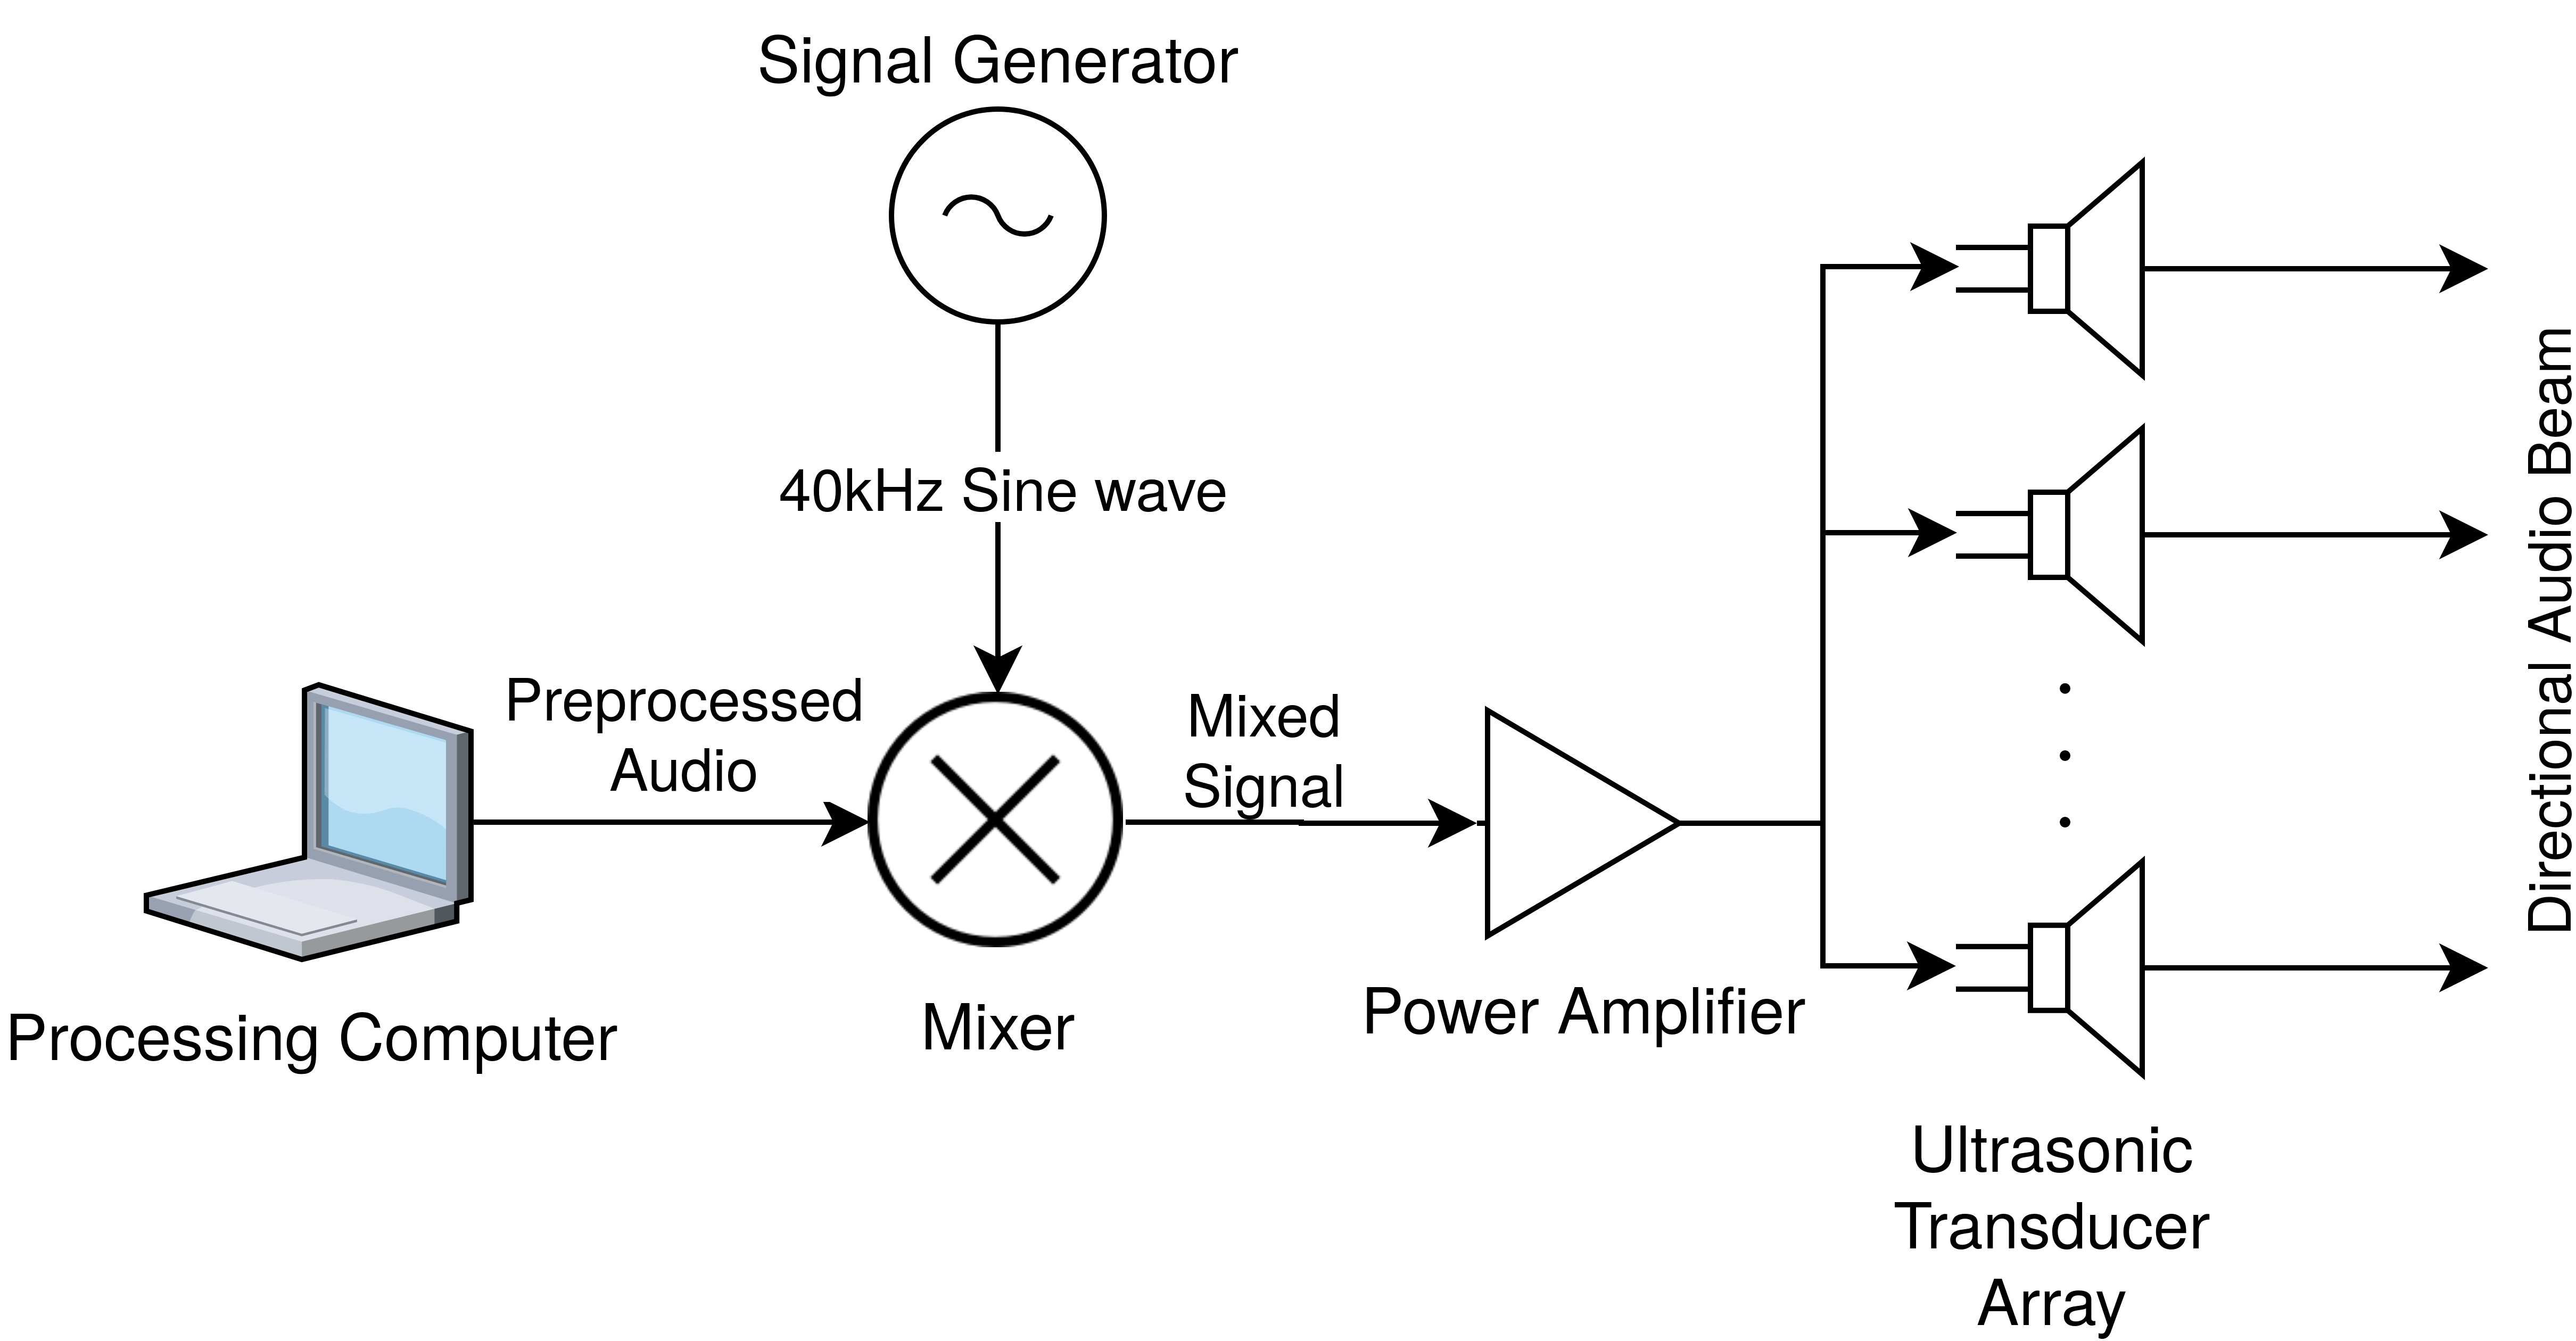
\includegraphics[width=0.8\textwidth]{Figures/Design/HighlevelSystemDesign.png}
    \caption{High level system design for the directional audio system}
    \label{fig:highleveldesign}
\end{figure}
The system begins by pre-processing audio using a specially developed julia program which applies the appropriate mathematical functions to a baseband audio clip and outputs the signal through the laptops audio jack.\\
This pre-processed signal is then mixed with a 40 kHz sine wave generated by a signal generator and passed into an amplifier. The amplifier increases the voltage swing of the mixed signal while having sufficient current to drive the ultrasonic transducers.\\
The ultrasonic transducers are connected in parallel with each other and thus all receive the same signal from the power amplifier. The transducers are packed into a densely packed array to provide a more more uniform transducer aperture which emits the input signal into the environment.

\subsection{Pre-processing subsystem design}
The pre-processing occurs in the form of a julia program which applies the mathematical functions shown in figure \ref{fig:sigpreprocessflow}. The program takes in a sampled signal $x_{in}(t)$ which is then shifted to the centre crossing by subtraction of its average value. The function then undertakes a sample wise double integral and is then raised above the centre crossing so only positive values remain. The square root of the function is then taken and the signal is then output into through the audio port of the laptop.
\begin{figure}[ht!]
    \centering
    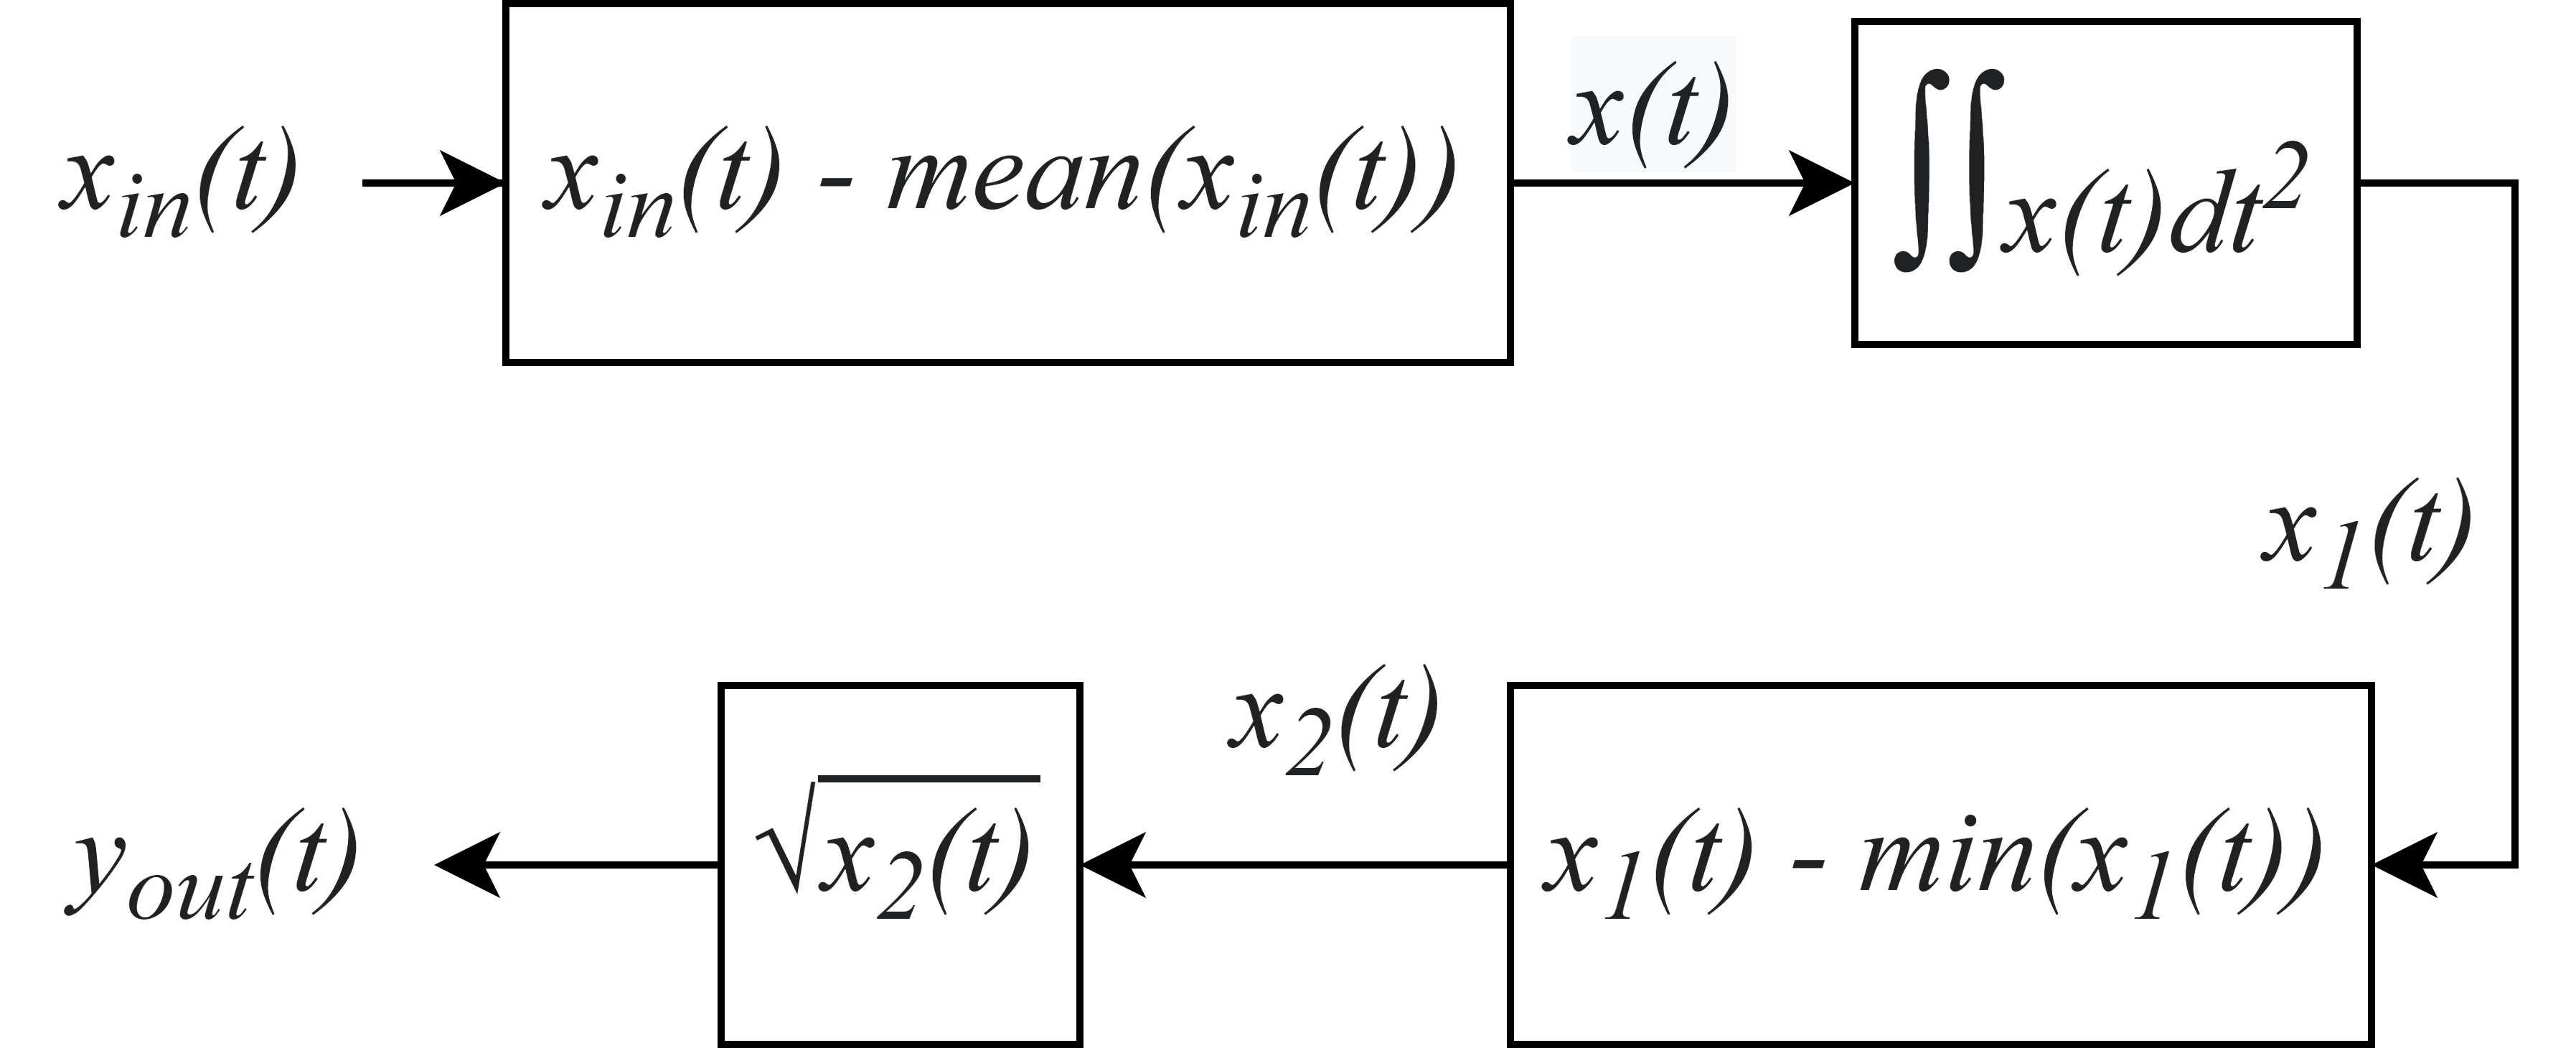
\includegraphics[width=0.7\textwidth]{Figures/Design/Preprocessing Design.png}
    \caption{Signal Pre-processing flowchart}
    \label{fig:sigpreprocessflow}
\end{figure}


\subsection{Mixer design}
The purpose of the mixer is to produce an amplitude modulated output of the carrier wave signal and the pre-processed audio signal. This can be done quite easily with the AD633 analogue multiplier with low cost supporting circuitry using the linear amplitude modulator circuit from the AD633 datasheet. The AD633 has the internal functional configuration shown in figure \ref{fig:mixerfunc} where X and Y are multiplied and the result is produced on output W.

\begin{figure}[ht!]
    \centering
    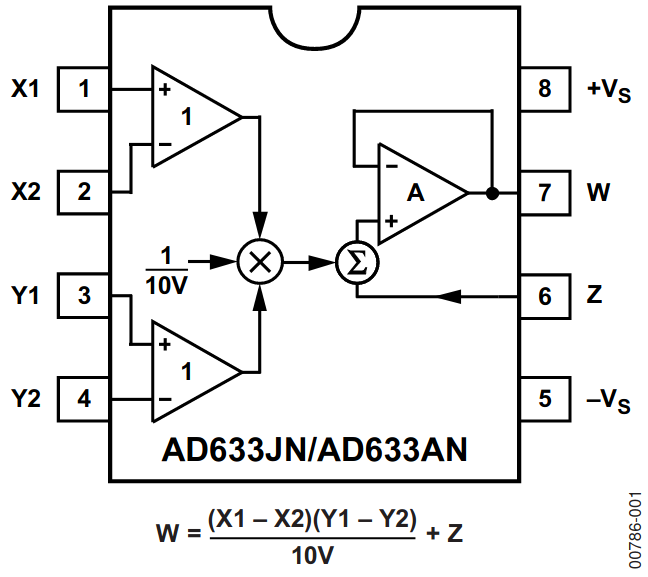
\includegraphics[width=0.5\textwidth]{Figures/Design/Mixer/ad633Intr.png}
    \caption{AD633 Functional diagram}
    \label{fig:mixerfunc}
\end{figure}

Analogue devices has a SPICE description of this components which was imported into LTSpice and used in the circuit shown in figure \ref{fig:amCirc}. The circuit is an implementation of the linear amplitude modulator reference circuit found in the AD633 datasheet and was adapted with relevant signal inputs (Vin, Vcarrier) to simulate the AD633's output (Vout).

\begin{figure}[ht!]
    \centering
    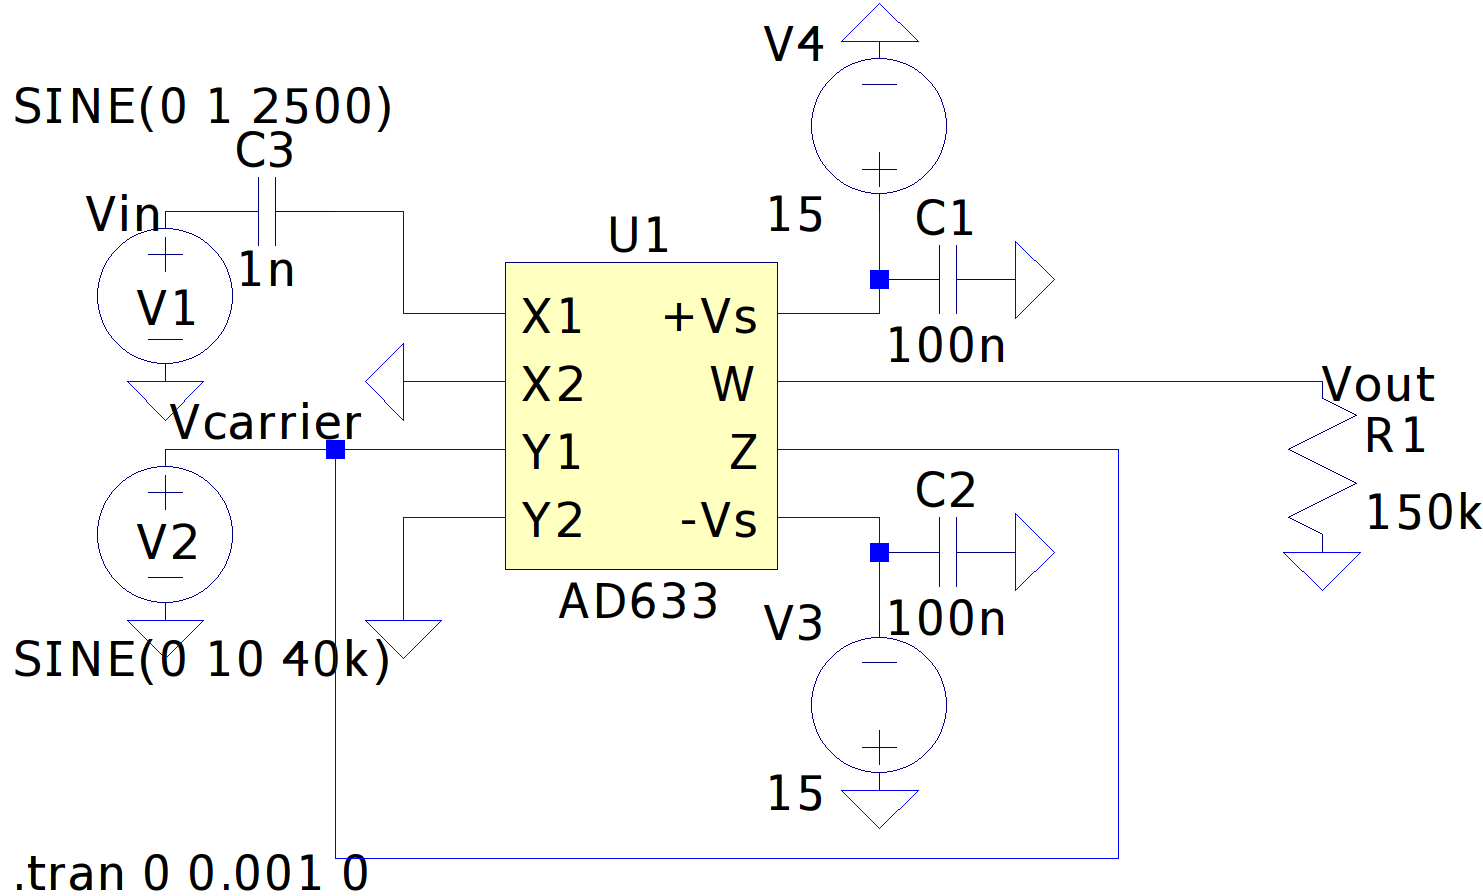
\includegraphics[width=0.7\textwidth]{Figures/Design/Mixer/ad633mixer.png}
    \caption{LTSpice circuit for AD633 Linear Amplitude Modulator}
    \label{fig:amCirc}
\end{figure}

\subsubsection{Mixer simulations}
To verify the design works as intended with the systems input signals, a 40 kHz carrier with a 10V amplitude is connected to the Y input while a 2.5 kHz test tone is connected through a decoupling capacitor to the X input. The output (W) is connected to a 150k resistor to simulate the expected load of the amplifier input. The expect functional result of this configuration is shown in equation \ref{eqn:mixSim}. Since X2 and Y2 are grounded (0V) they fall away and a double side band large carrier amplitude modulation function is the result.
\begin{equation}\label{eqn:mixSim}
    W = \frac{(V_{in})(V_{carrier})}{10} + V_{carrier}
\end{equation}

Figure \ref{fig:mixervinvout} demonstrates the time domain expression for the output voltage across R1 as well as the input voltage $V_{in}$. The modulating amplitude is 1V and the carrier amplitude is 10V which are ten times the value presented to the internal multiplier as shown in figure \ref{fig:mixerfunc}. The simulation reveals that the output has a maximum amplitude of 2.9V and a minimum amplitude of 1.1V. This output doesn't produce an ideal modulation index of 100\% which would produce a stronger signal strength.

\begin{figure}[ht!]
    \centering
    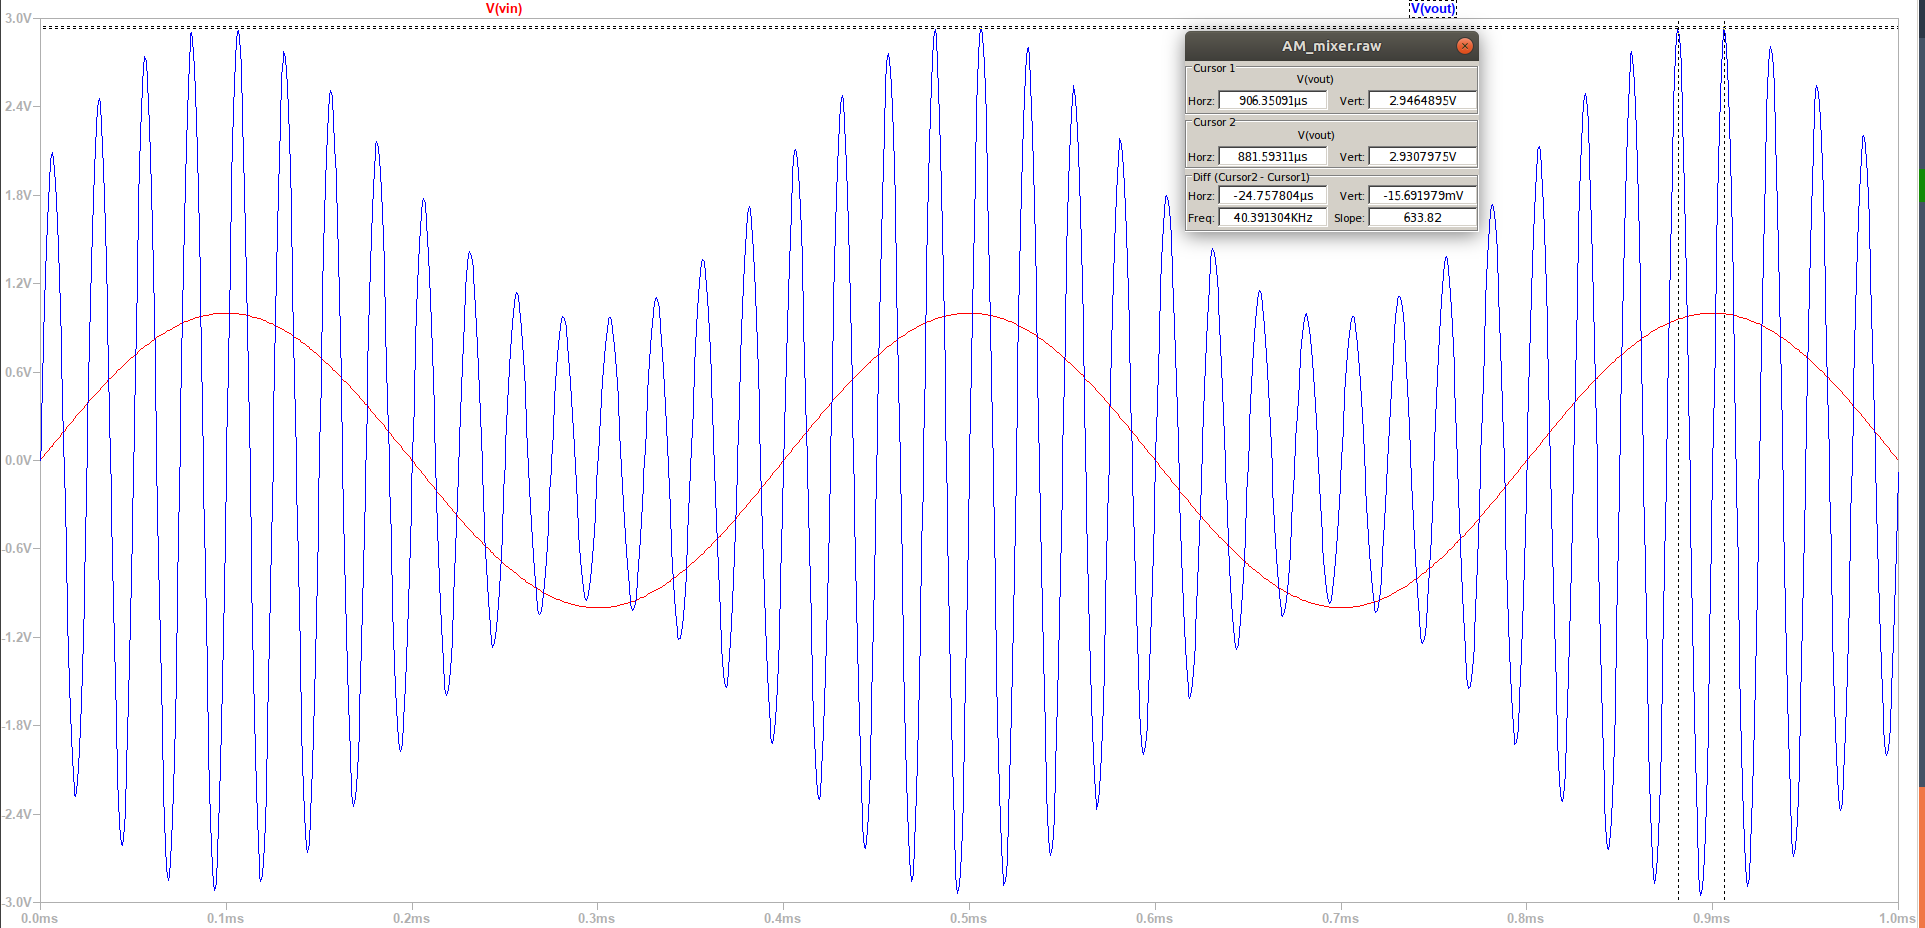
\includegraphics[width=0.7\textwidth]{Figures/Design/Mixer/mixerVinVoutFc.png}
    \caption{Input and output voltage of the AD633 based linear amplitude modulator}
    \label{fig:mixervinvout}
\end{figure}

To achieve a modulation index closer to 100\%, the input voltage of the modulation signal would have to be increased. To illustrate this effect, the amplitude of $V_{in}$ was adjusted until the peak voltage of the negative half cycle of the output is as close as feasibly possible to the zero crossing. Figure \ref{fig:mixervin195} demonstrates $V_{in}$ set to a amplitude of 1.95V which achieves a lower voltage of 50mV. This is very close to the zero crossing and risks causing over-modulation if the input voltage spikes. The result of the input amplitude raising above 1.95V is shown in figure \ref{fig:mixervin25} where the input amplitude is set to 2.5V and results in the outputs' negative half-cycle peaking at 500mV which is the result of over-modulation.

\begin{figure}[ht!]
    \centering
    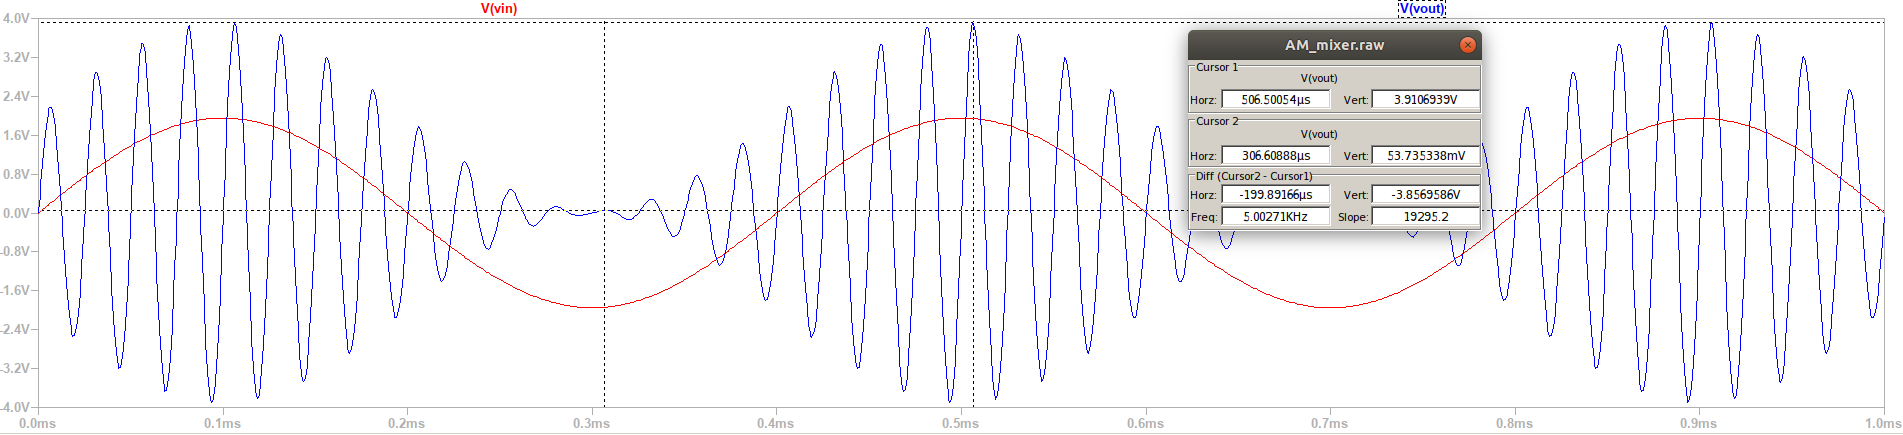
\includegraphics[width=0.7\textwidth]{Figures/Design/Mixer/195Vm10Vc.png}
    \caption{Input and output voltage of the AD633 with $V_{in}$ at 1.95V amplitude demonstrating ideal modulation index}
    \label{fig:mixervin195}
\end{figure}

\begin{figure}[ht!]
    \centering
    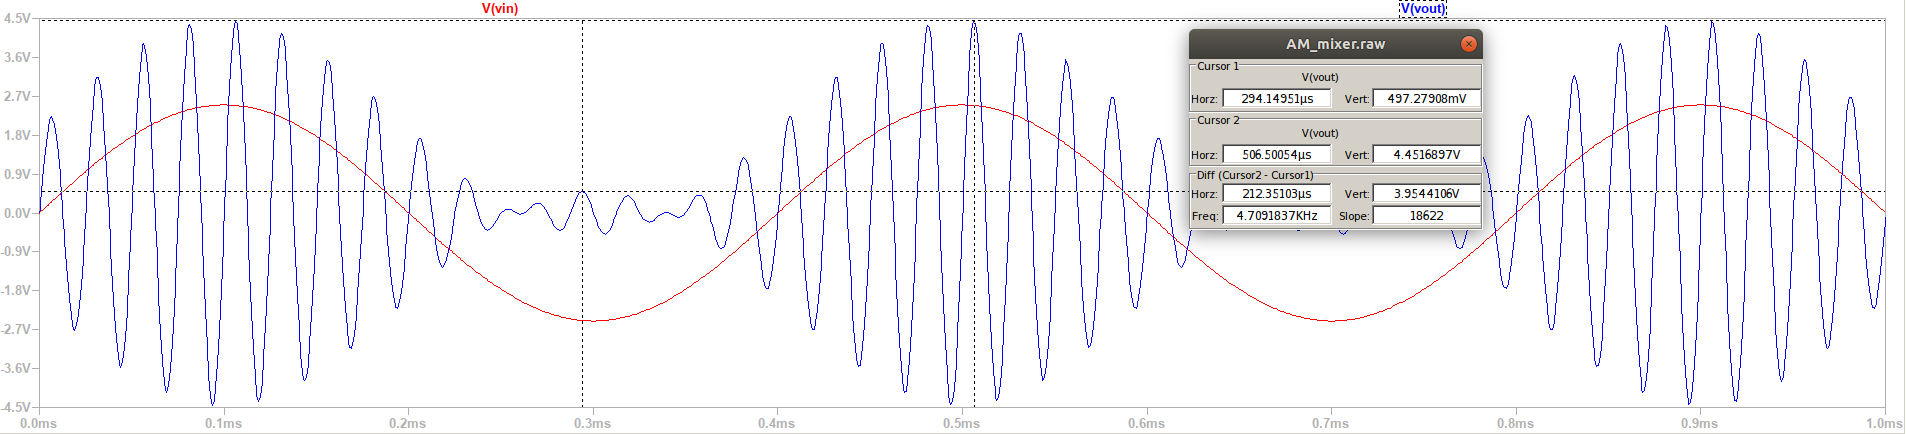
\includegraphics[width=0.7\textwidth]{Figures/Design/Mixer/25Vm10VcOvermod.png}
    \caption{Input and output voltage of the AD633 with $V_{in}$ at 2.5V amplitude demonstrating over-modulation}
    \label{fig:mixervin25}
\end{figure}

To achieve a modulation index close to 100\% without risking over-modulation, the input amplitude is set to 1.75V as shown in figure \ref{fig:mixervin175}. The resulting output reaches a minimum amplitude of 245mV with a maximum amplitude of 3.70V. Since the output amplitude without a modulating signal is 2V ($A_{Carrier}$), the modulation index can be calculated with equation \ref{eqn:modIndex} and results in an approximate modulation index of 85\%.
\begin{equation}\label{eqn:modIndex}
    m = \frac{A_{Env\_peak}}{A_{Carrier}} - 1
\end{equation}
While a modulation index of 85\% would be ideal, it is not attainable since the maximum amplitude the laptop's audio output can reach is limited to 1V. Given the prior maximum of 2.95V, this limitation produces an approximate maximum modulation index of 48\%.
\begin{figure}[ht!]
    \centering
    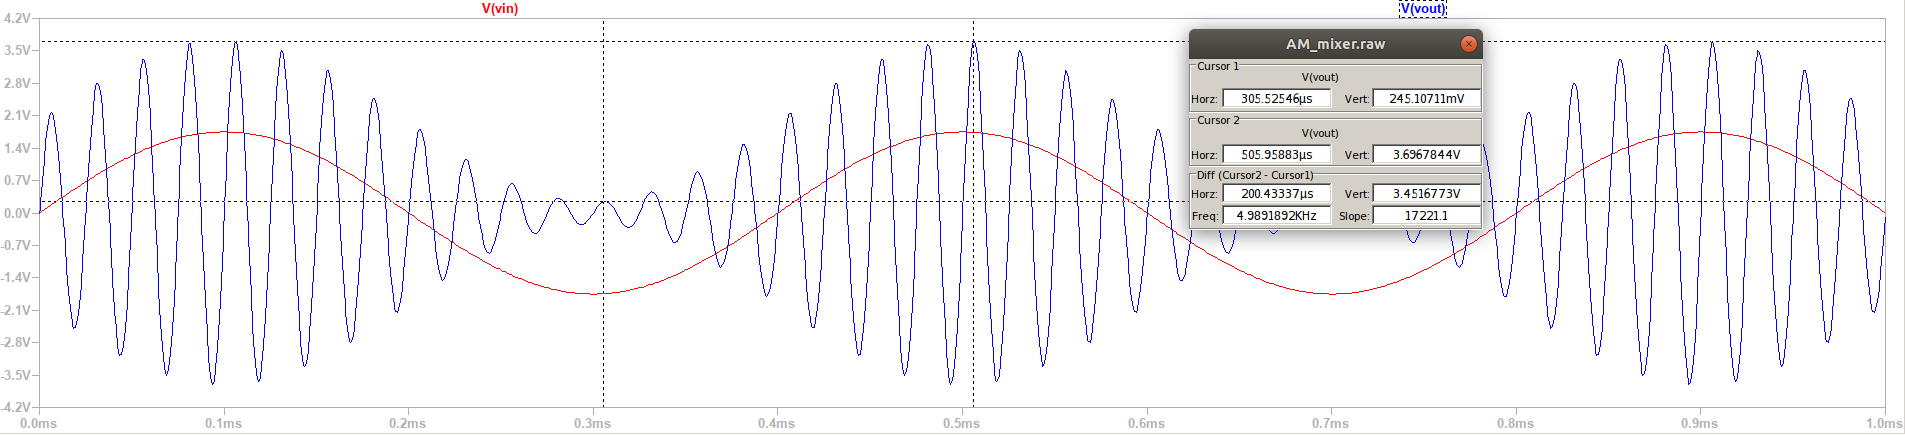
\includegraphics[width=0.7\textwidth]{Figures/Design/Mixer/175Vm10Vc.png}
    \caption{Input and output voltage of the AD633 with $V_{in}$ at 1.75V amplitude}
    \label{fig:mixervin175}
\end{figure}


\newpage
\subsection{Amplifier design}
The amplifier's purpose in the system is to increase the peak-to-peak voltage of the output signal for the ultrasonic transducers while providing sufficient current to the transducers. During existing amplifier research the Texas Instruments LM380 was chosen. Main aspects about this audio power amplifier that drove this decision included the wide supply voltage range of up to 22V, 2.5W output power and flat gain curve with a bandwidth of 100 kHz. Since the device is expected to operate around 40 kHz, the amplifier needs to respond linearly at this frequency.\\
The supporting circuitry for this amplifier was adapted from the phono amplifier example application circuit within the LM380's datasheet and simulated in LTSpice XVII.

\begin{figure}[ht!]
    \centering
    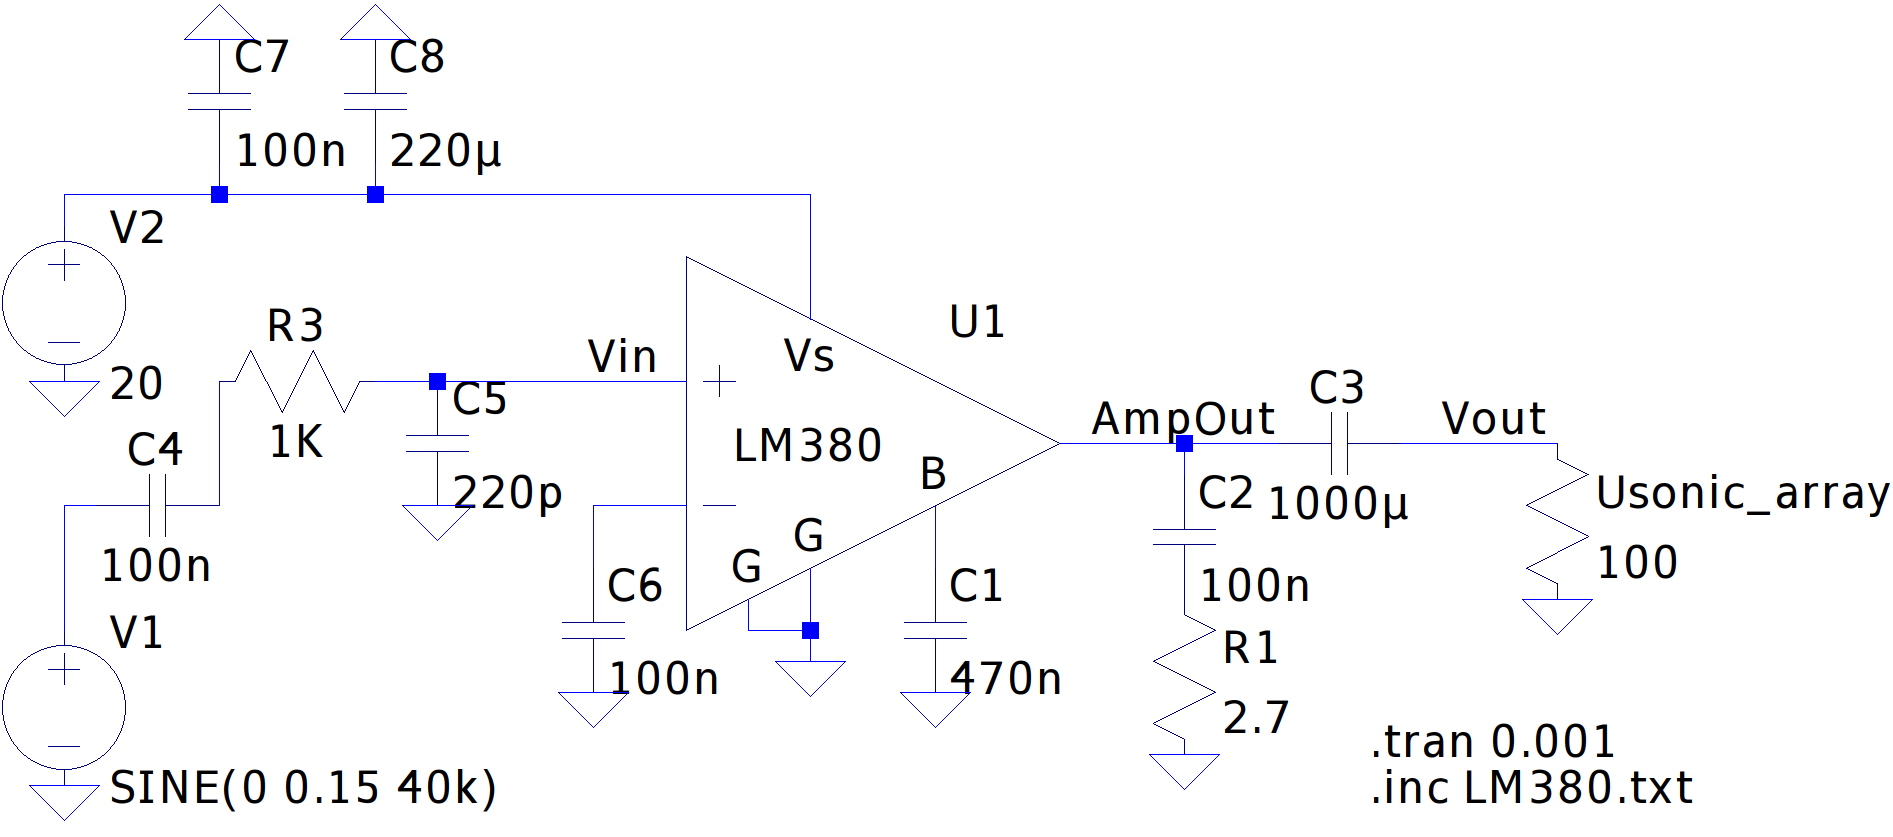
\includegraphics[width=\textwidth]{Figures/Design/amplifier/lm380circwhitestable.png}
    \caption{The circuit design adapted from phono amplifier example application within LM380 datasheet}
    \label{fig:lm380circ}
\end{figure}

Figure \ref{fig:lm380circ} shows the LM380 amplifier along with the recommended circuitry for stable operation. An assumption was made to represent the ultrasonic array as a 100 $\Omega$ resistor as from investigating the datasheet of a ultrasonic transducer, a single transducer was found too have a equivalent resistance of 1000$\Omega$ at 40 kHz. When connecting 10 of these transducers in parallel the resistance is estimated to reduce to 100 $\Omega$, hence the load in figure \ref{fig:lm380circ}. If transducer array were increased to 20, this load would half down to 50$\Omega$ and would consume approximately double the power.

\subsubsection{Amplifier simulations}
To verify whether the circuit in figure \ref{fig:lm380circ} would achieve the desired gain and at the intended carrier frequency, simulations were done to test the input to output voltage (gain) as well as the output current of the LM380.

\begin{figure}[ht!]
    \centering
    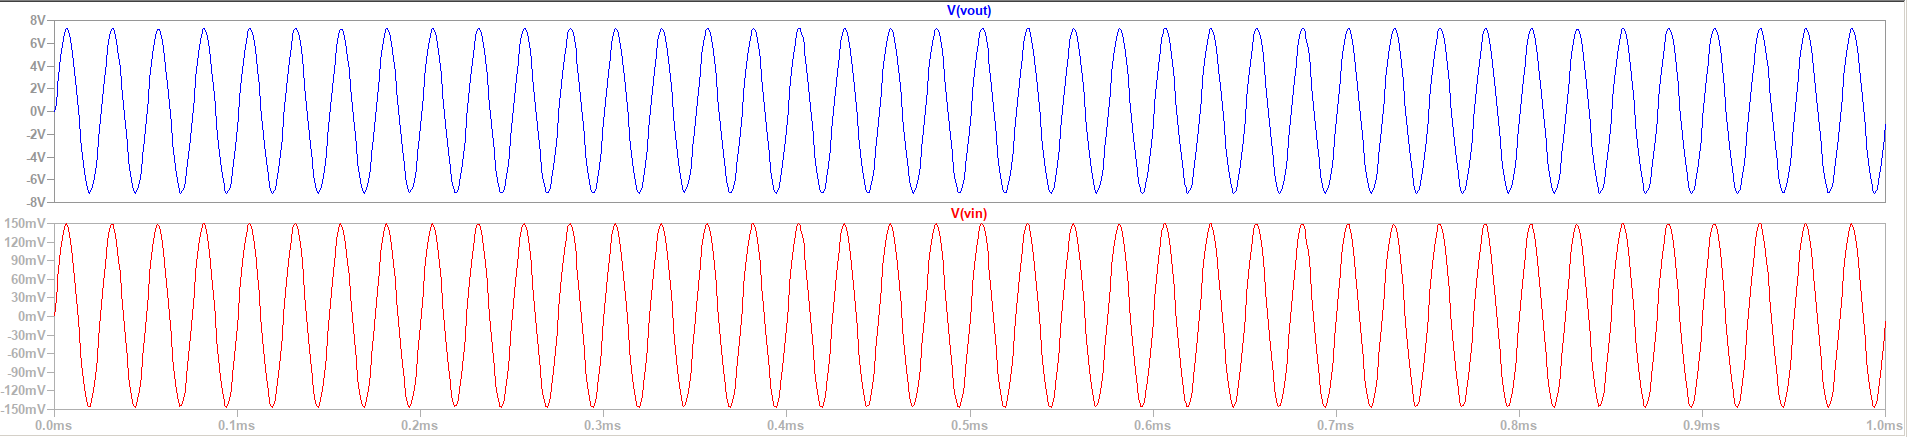
\includegraphics[width=\textwidth]{Figures/Design/amplifier/vinvout.png}
    \caption{Input voltage versus output voltage of the LM380 at 40 kHz}
    \label{fig:lm380inoutsim}
\end{figure}
Figure \ref{fig:lm380inoutsim} shows the input voltage to the LM380 and the output voltage across the ultrasonic transducer array. The input voltage is $300mV_{p-p}$ while the output across the transducers is $14V_{p-p}$, resulting in a voltage gain of 46.7. Note however that this output is passed through a decoupling capacitor to centre it on the zero crossing. To investigate the upper limit of the peak-to-peak voltage swing, a measurement is made before the decoupling capacitor and the reading is shown in figure \ref{fig:lm380outsim}.

\begin{figure}[ht!]
    \centering
    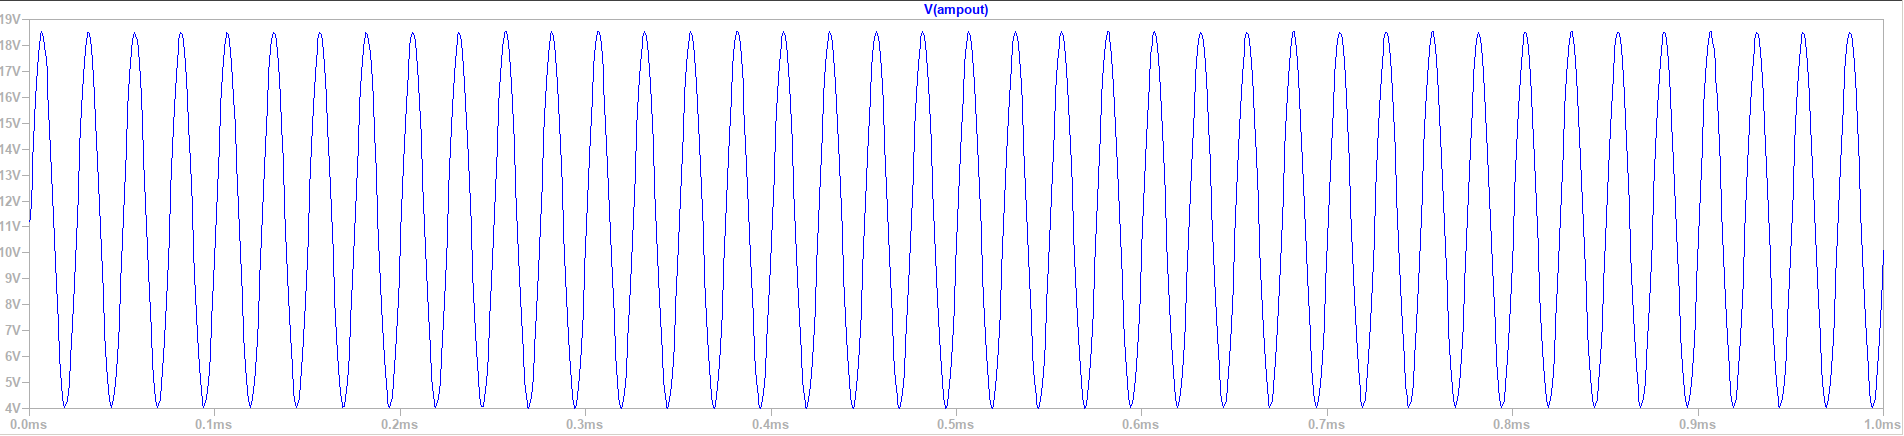
\includegraphics[width=\textwidth]{Figures/Design/amplifier/vamp.png}
    \caption{Output voltage on the output pin of the LM380 at 40 kHz}
    \label{fig:lm380outsim}
\end{figure}

From figure \ref{fig:lm380outsim} one can see the output voltage swings between 4V and 18.5V with a supply voltage of 20V. The LM380 is rated for a maximum output voltage swing of $14V_{p-p}$ and as a result it is expected the supply voltage should not go lower than 15V since that would result in the output hitting the rails of the supply and produce added noise and clipping. To test this assumption, a decreasing supply voltage was simulated to reduce the supply voltage from 20V to 15V. Figure \ref{fig:lm380outVsSupply} demonstrates the simulated relationship between supply voltage and the resultant output voltage swing of the LM380 amplifier.

\begin{figure}[ht!]
    \centering
    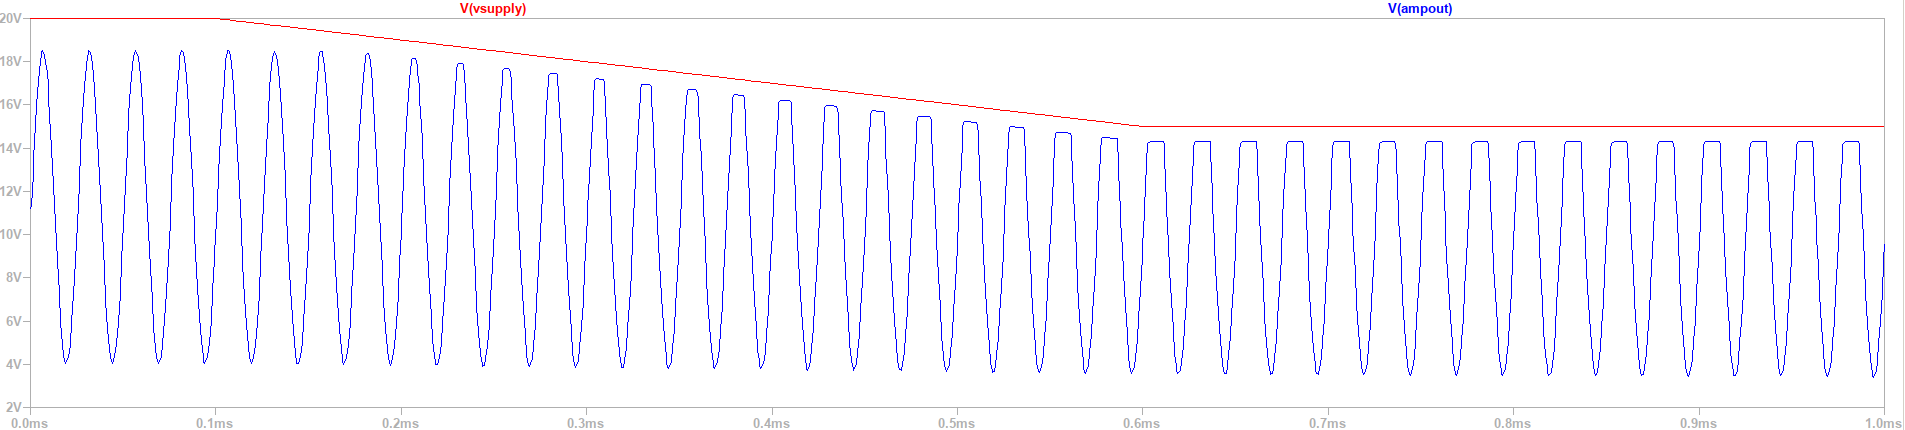
\includegraphics[width=\textwidth]{Figures/Design/amplifier/vsupplyvsVampOut.png}
    \caption{Output voltage on the output pin of the LM380 compared to supply voltage}
    \label{fig:lm380outVsSupply}
\end{figure}

The simulation reveals that there needs to be at least 6V more than the 14V peak to peak output swing to achieve an undistorted output waveform with an input voltage of $300mV_{p-p}$. This means the supply voltage for the LM380 should remain at 20V to mitigate this clipping effect. Alternatively if the input peak-to-peak voltage is reduced to $200mV_{p-p}$ this could reduce the required supply voltage. A simulation of reducing the input voltage to $200mV_{p-p}$ is shown in figure \ref{fig:lm380outVsSupply100mvin}.

\begin{figure}[ht!]
    \centering
    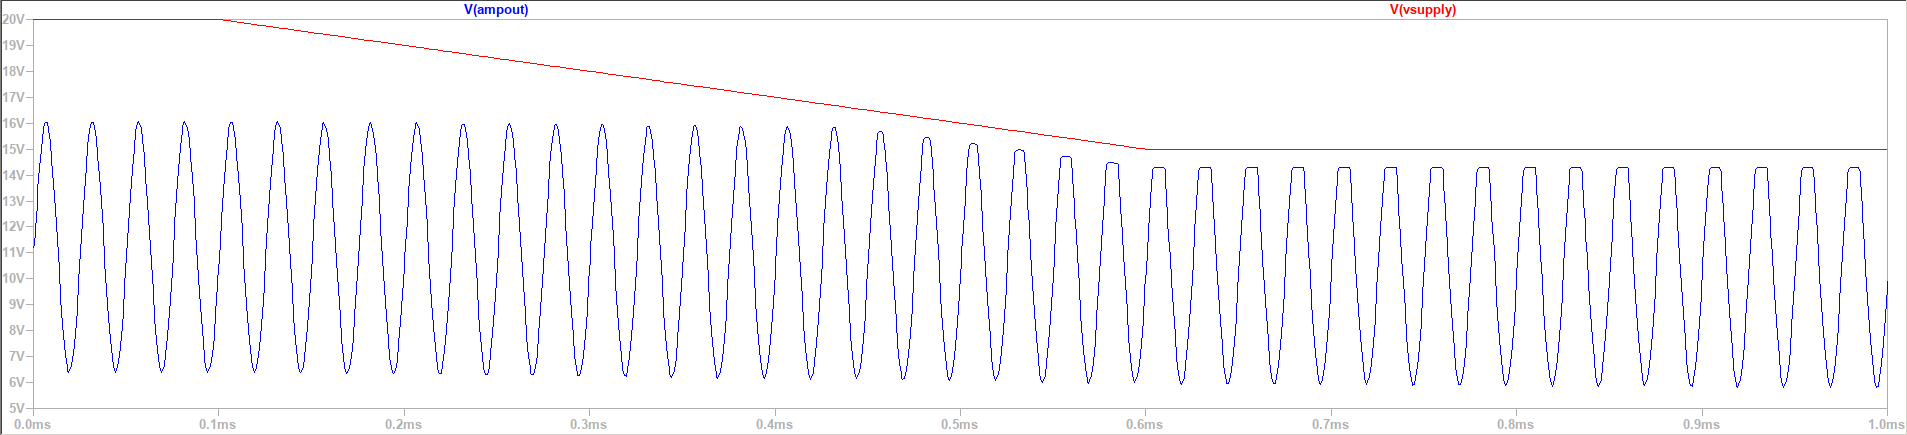
\includegraphics[width=\textwidth]{Figures/Design/amplifier/voutVsvsupplyInput100mv.png}
    \caption{Output voltage on the output pin of the LM380 compared to supply voltage with a reduced peak-to-peak input voltage}
    \label{fig:lm380outVsSupply100mvin}
\end{figure}

The results of reducing the input voltage show that the LM380 amplifier can indeed operate at a lower voltage without clipping its output, however; this is due to a reduced peak-to-peak output voltage of $10V_{p-p}$. This results in a overall voltage gain of the amplifier of 50 which is larger than before, but it also reduces the peak-to-peak voltage at the output which is directly proportional to more transducer movement and thus, a higher sound pressure level in the environment.\\
Finally the output current was simulated by measuring the current passing through the simulated ultrasonic load. Figure \ref{fig:lm380Iout} demonstrates a peak-to-peak current of 140mA while producing a $14V_{p-p}$ voltage across the ultrasonic load. This results in a total power of 1.39W through the load when using RMS voltage and current in the calculation which is well within the 2.5W maximum power the LM380 is rated for. If the load were to reduce due to more transducer being added in parallel, the consumed power would increase. As long as the peak-to-peak current remains below 252mA, the amplifier is operating within the specification of its datasheet. This current translates to a load of approximately 55$\Omega$ which results in a parallel transducer configuration of 19 to 21 transducers.

\begin{figure}[ht!]
    \centering
    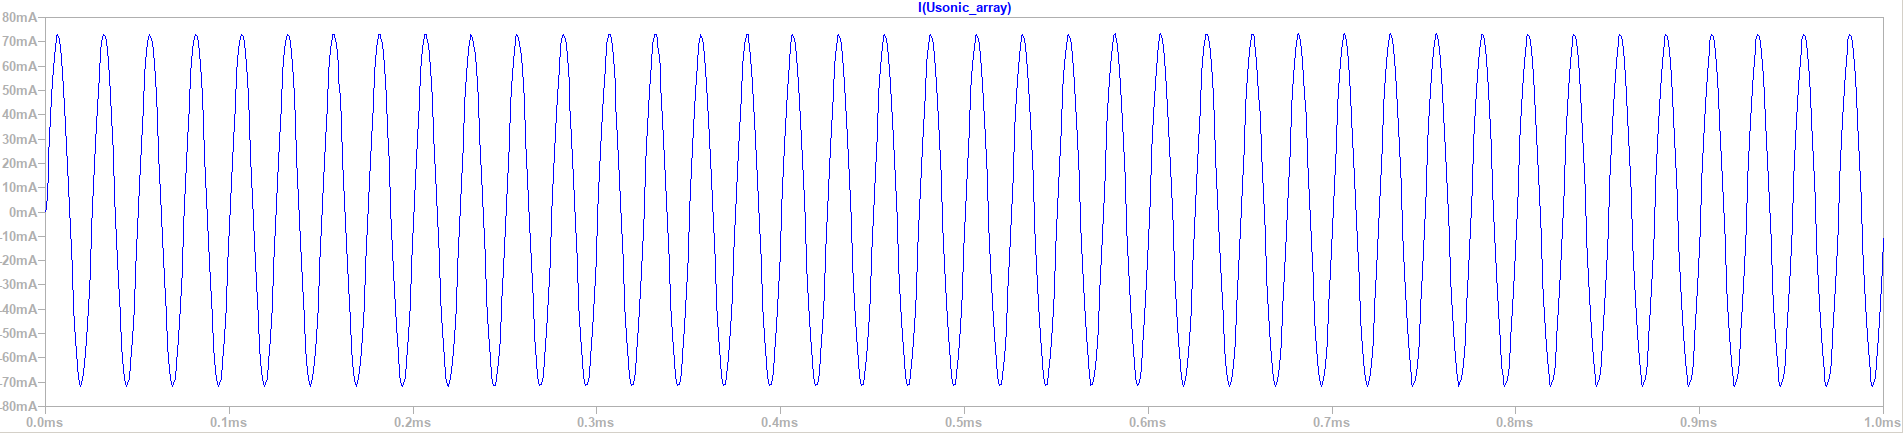
\includegraphics[width=\textwidth]{Figures/Design/amplifier/ioutusonic.png}
    \caption{Output current of the LM380 through the simulated ultrasonic transducer array}
    \label{fig:lm380Iout}
\end{figure}

\subsection{Ultrasonic array design}
The design of the directional speaker's ultrasonic array involves packing the transducers as densely as possible while maintaining a relatively circular aperture to ensure a uniform beam shape.
\subsubsection{Element packing}
To maximise the directivity of the ultrasonic array, the distance between the centroids of all the neighbouring transducers must be minimised. This forms a more densely packed element array and thus, a more uniform beam shape.
To maximise the density of the transducers, a class of optimisation called packing can be used. The aim of packing is to insert geometric shapes in a container as densely as possible.\\
To evaluate possible transducer packing designs, a packing tool provided by Wolfram Alpha for 2D geometric packing \cite{alpha_2018} is used. The tool allows for dimension definition of the container (object to contain the packed geometry) as well as the packing elements (objects to be packed in the container). The container is set to varying dimensions while keeping the packing elements radius at 0.8cm as specified by the transducer's datasheet.\\
Packing consists of many different methods involving a particularly type of symmetry. As shown in figure \ref{fig:densest4.1}, a circular container of 4.1cm can be packed with 20 transducers producing a 76.15\% filled fraction. While this may appear viable, the imbalanced placement of the transducers which may produce an inconsistent beam shape resulting in a single stronger side lobe on one side of the aperture than the others.
\newpage
\begin{figure}[ht!]
\centering

    \begin{minipage}{0.4\textwidth}
    \centering
    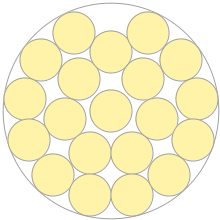
\includegraphics[width= \textwidth]{Figures/Packing/DensestPacking_r0.8_R4.1.png}
    \caption{Densest possible pattern in a circle of radius 4.1cm}
    \label{fig:densest4.1}
    \end{minipage}\hfill
    \begin{minipage}{0.4\textwidth}
    \centering
    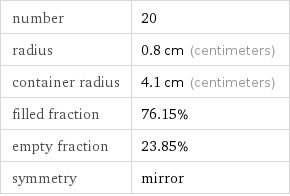
\includegraphics[width= \textwidth]{Figures/Packing/DensestPacking_r0.8_R4.1_packingPercent.png}
    \caption{Densest density information for a circle of radius 4.1cm}
    \label{fig:densest4.1_packinginfo}
    \end{minipage}
    
\end{figure}

\begin{figure}[ht!]
\centering

    \begin{minipage}{0.4\textwidth}
    \centering
    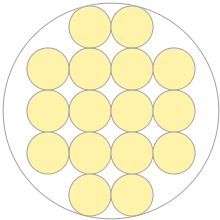
\includegraphics[width= \textwidth]{Figures/Packing/SquarePacking_r0.8_R4.1.png}
    \caption{Rectangular packing pattern in a circle of radius 4.1cm}
    \label{fig:square4.1}
    \end{minipage}\hfill
    \begin{minipage}{0.4\textwidth}
    \centering
    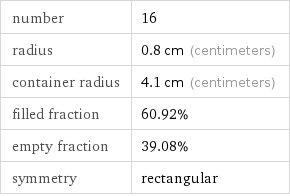
\includegraphics[width= \textwidth]{Figures/Packing/SquarePacking_r0.8_R4.1_packingPercent.png}
    \caption{Density information with square packing for a circle of radius 4.1cm}
    \label{fig:squaret4.1_packinginfo}
    \end{minipage}
    
\end{figure}

Investigating an alternative type of symmetry revealed the rectangular packed result in figure \ref{fig:square4.1}. This suffers from having a lower filled fraction of 60.92\% using the same 4.1cm container radius as before but shows more uniformity in transducer placement.\\

Another form of symmetry called inversion is investigated in figure \ref{fig:hex4.1} using the 4.1cm container radius. This configuration results in a hexagonally packed transducer placement pattern and has a filled fraction of 72.34\%. The pattern allows for 19 transducers to fit within the container while maintaining even spacing between the transducers. This would result in a more uniform beam shape than the packing used in figure \ref{fig:densest4.1} as the distance between the transducers is minimised on all sides.


\begin{figure}[ht!]
\centering

    \begin{minipage}{0.4\textwidth}
    \centering
    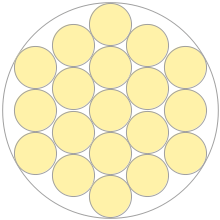
\includegraphics[width= \textwidth]{Figures/Packing/hexagonalPacking_r0.8_R4.1.png}
    \caption{Hexagonal packing pattern in a circle of radius 4.1cm}
    \label{fig:hex4.1}
    \end{minipage}\hfill
    \begin{minipage}{0.4\textwidth}
    \centering
    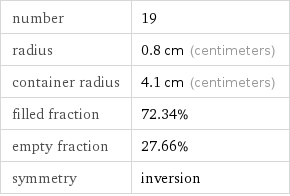
\includegraphics[width= \textwidth]{Figures/Packing/hexagonalPacking_r0.8_R4.1_packingPercent.png}
    \caption{Density information with hexagonal packing for a circle of radius 4.1cm}
    \label{fig:hex4.1_packinginfo}
    \end{minipage}
    
\end{figure}

To see the effect of increased container size, the container was increased slightly to a radius of 4.5cm. Unfortunately this results in erratic placement of transducers for the mirror and inversion symmetry types shown in figures \ref{fig:dense4.5} and \ref{fig:hex4.5} respectively which is undesirable for producing a uniform beam shape. The container size increase did however produce a favourable result for the square packed symmetry shown in figure \ref{fig:sqr4.5}, featuring a filled fraction of 66.37\% with uniform placement of transducers.

\begin{figure}[ht!]
\centering

    \begin{minipage}{0.4\textwidth}
    \centering
    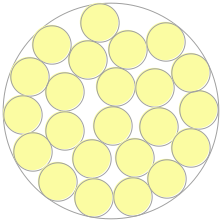
\includegraphics[width= \textwidth]{Figures/Packing/DensestPacking_r0.8_R4.5.png}
    \caption{Densest packing pattern in a circle of radius 4.5cm}
    \label{fig:dense4.5}
    \end{minipage}\hfill
    \begin{minipage}{0.4\textwidth}
    \centering
    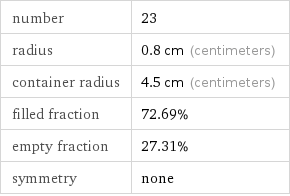
\includegraphics[width= \textwidth]{Figures/Packing/DensestPacking_r0.8_R4.5_packingPercent.png}
    \caption{Density information with densest packing for a circle of radius 4.5cm}
    \label{fig:dense4.5_packinginfo}
    \end{minipage}
    
\end{figure}

\begin{figure}[ht!]
\centering

    \begin{minipage}{0.4\textwidth}
    \centering
    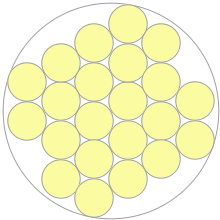
\includegraphics[width= \textwidth]{Figures/Packing/hexagonalPacking_r0.8_R4.5.png}
    \caption{Hexagonal packing pattern in a circle of radius 4.5cm}
    \label{fig:hex4.5}
    \end{minipage}\hfill
    \begin{minipage}{0.4\textwidth}
    \centering
    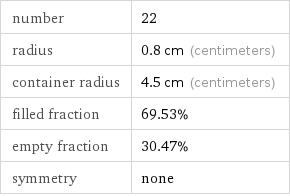
\includegraphics[width= \textwidth]{Figures/Packing/hexagonalPacking_r0.8_R4.5_packingPercent.png}
    \caption{Density information with hexagonal packing for a circle of radius 4.5cm}
    \label{fig:hex4.5_packinginfo}
    \end{minipage}
    
\end{figure}


\begin{figure}[ht!]
\centering

    \begin{minipage}{0.4\textwidth}
    \centering
    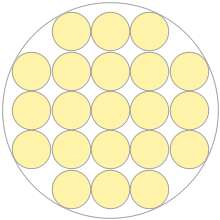
\includegraphics[width= \textwidth]{Figures/Packing/SquarePacking_r0.8_R4.5.png}
    \caption{Square packing pattern in a circle of radius 4.5cm}
    \label{fig:sqr4.5}
    \end{minipage}\hfill
    \begin{minipage}{0.4\textwidth}
    \centering
    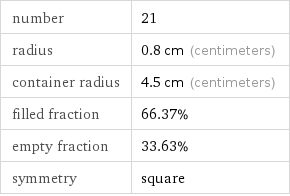
\includegraphics[width= \textwidth]{Figures/Packing/SquarePacking_r0.8_R4.5_packingPercent.png}
    \caption{Density information with square packing for a circle of radius 4.5cm}
    \label{fig:sqr4.5_packinginfo}
    \end{minipage}
    
\end{figure}
\newpage

In conclusion, two of these layouts show potential. For a container radius of 4.1cm, the hexagonally packed array shown in figure \ref{fig:hex4.1} is most effective due to its high filled fraction of 72.34\% resulting in closer spacing of transducers. It does however only contain 19 transducers which is near the upper limit of the amplifier's output power but risks producing a lower output sound pressure level than a higher transducer count solution would achieve. By increasing the radius to 4.5cm, a higher transducer count of 21 is achieved in the square packed solution shown in figure \ref{fig:sqr4.5} albeit with a lower filled fraction of 66.37\%. The additional output power potential of the 4.5cm radius square packed array is more appealing for this application as the audible sound produced by these transducers is significantly low, thus maximising the output power of the array is a favourable design choice.

%commented this out because it doesn't serve much purpose
\begin{comment}
\begin{figure}[h]
\centering

    \begin{minipage}{0.4\textwidth}
    \centering
    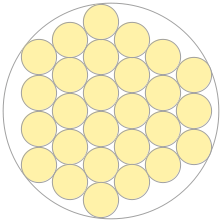
\includegraphics[width= \textwidth]{Figures/Packing/hexagonalPacking_r0.8_R4.9.png}
    \caption{Hexagonal packing pattern in a circle of radius 4.9cm}
    \label{fig:hex4.9}
    \end{minipage}\hfill
    \begin{minipage}{0.4\textwidth}
    \centering
    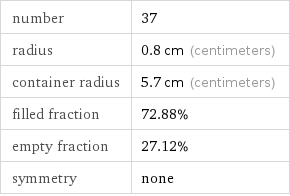
\includegraphics[width= \textwidth]{Figures/Packing/hexagonalPacking_r0.8_R4.9_packingPercent.png}
    \caption{Density information with hexagonal packing for a circle of radius 4.9cm}
    \label{fig:hex4.9_packinginfo}
    \end{minipage}
    
\end{figure}

\end{comment}

\newpage
\subsubsection{Array design simulations}
The purpose of creating the ultrasonic array is to maximise the directivity of the speaker system. To aid in choosing an appropriate array packing profile, some designs were simulated to illustrate the effect that transducer placement has on the radiated beam shape with the goal or reducing side lobes while maximising the main lobe.\\
The transducer patterns from figure \ref{fig:hex4.1} with hexagonal packing and figure \ref{fig:sqr4.5} with square packing were simulated and compared as their designs have symmetry which is required for a uniform beam pattern.\\
To start, a single transducer is modeled and its approximate beam shape simulated with use of a two-dimensional Fourier Transform.

\begin{figure}[h!]
\centering

    \begin{minipage}{0.4\textwidth}
    \centering
    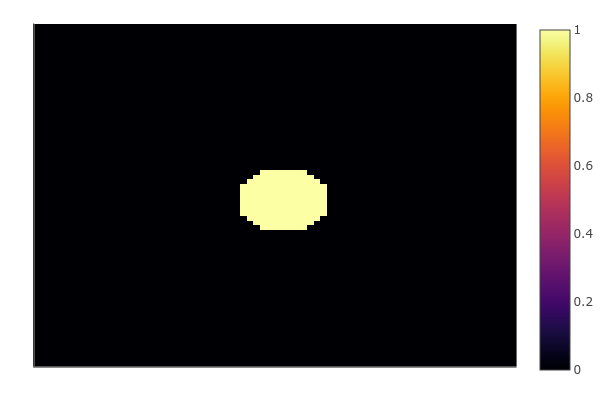
\includegraphics[width= \textwidth]{Figures/arraySim/single/element1.png}
    \caption{Single ultrasonic transducer element to be modeled}
    \label{fig:single_elem}
    \end{minipage}\hfill
    \begin{minipage}{0.4\textwidth}
    \centering
    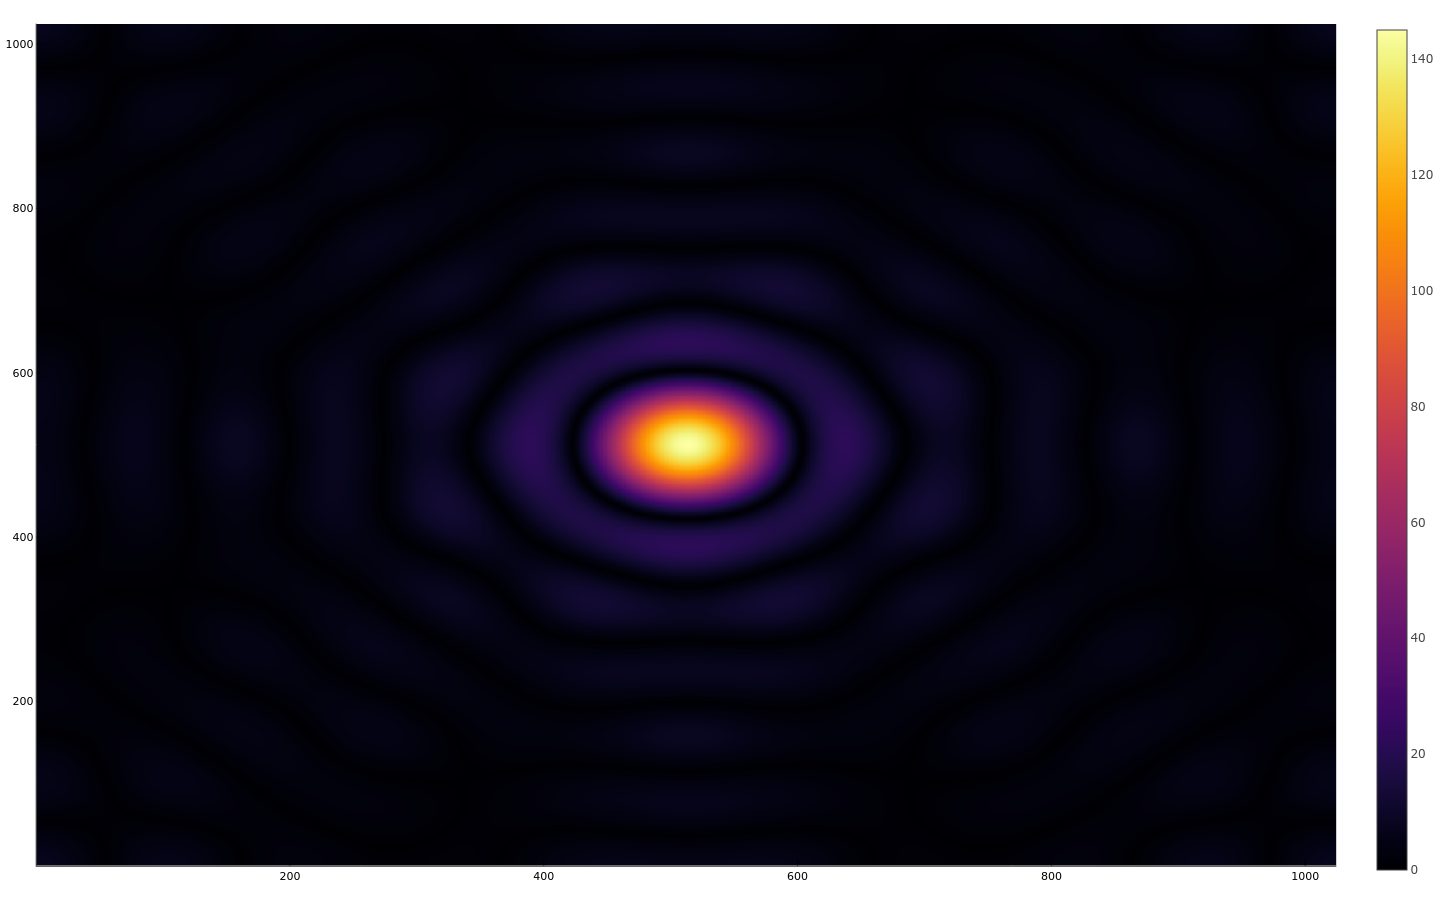
\includegraphics[width= \textwidth]{Figures/arraySim/single/beampat_top.png}
    \caption{Approximate beam shape of a single ultrasonic transducer (Bore-sight view)}
    \label{fig:single_elem_topBeam}
    \end{minipage}
    
\end{figure}
When viewed in three-dimensions, a single element produces the beam shape shown in figure \ref{fig:single_elem_3Dbeam}.
\begin{figure}[ht!]
    \centering
    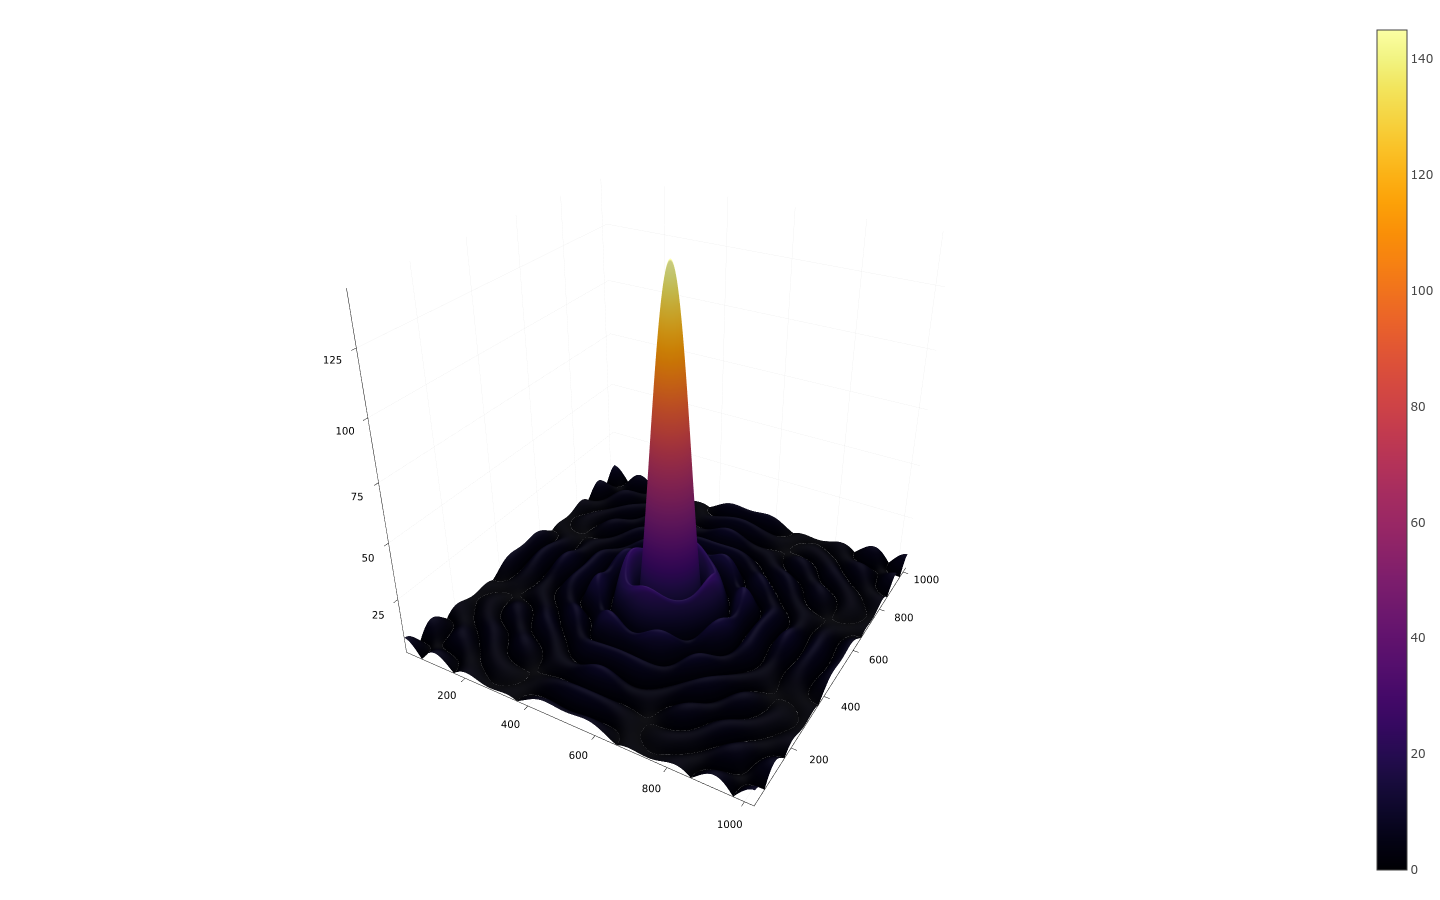
\includegraphics[width=0.7\textwidth]{Figures/arraySim/single/beampat3D.png}
    \caption{Approximate beam shape of a single ultrasonic transducer (3D view)}
    \label{fig:single_elem_3Dbeam}
\end{figure}
\newpage
Extrapolating the single element into both the hexagonal and square packed designs was done by estimating the spacing between transducers in each design and placing the elements according to this spacing. The square pattern is shown below in figure \ref{fig:sqr_elem} along with its bore-sight beam shape in figure \ref{fig:sqr_elem_topBeam}.
\begin{figure}[h!]
\centering

    \begin{minipage}{0.4\textwidth}
    \centering
    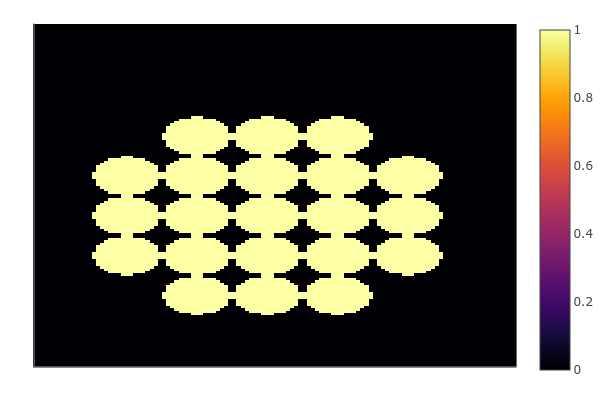
\includegraphics[width= \textwidth]{Figures/arraySim/sqr/arraylayoutcircular.png}
    \caption{Square packed ultrasonic transducer elements to be modeled}
    \label{fig:sqr_elem}
    \end{minipage}\hfill
    \begin{minipage}{0.4\textwidth}
    \centering
    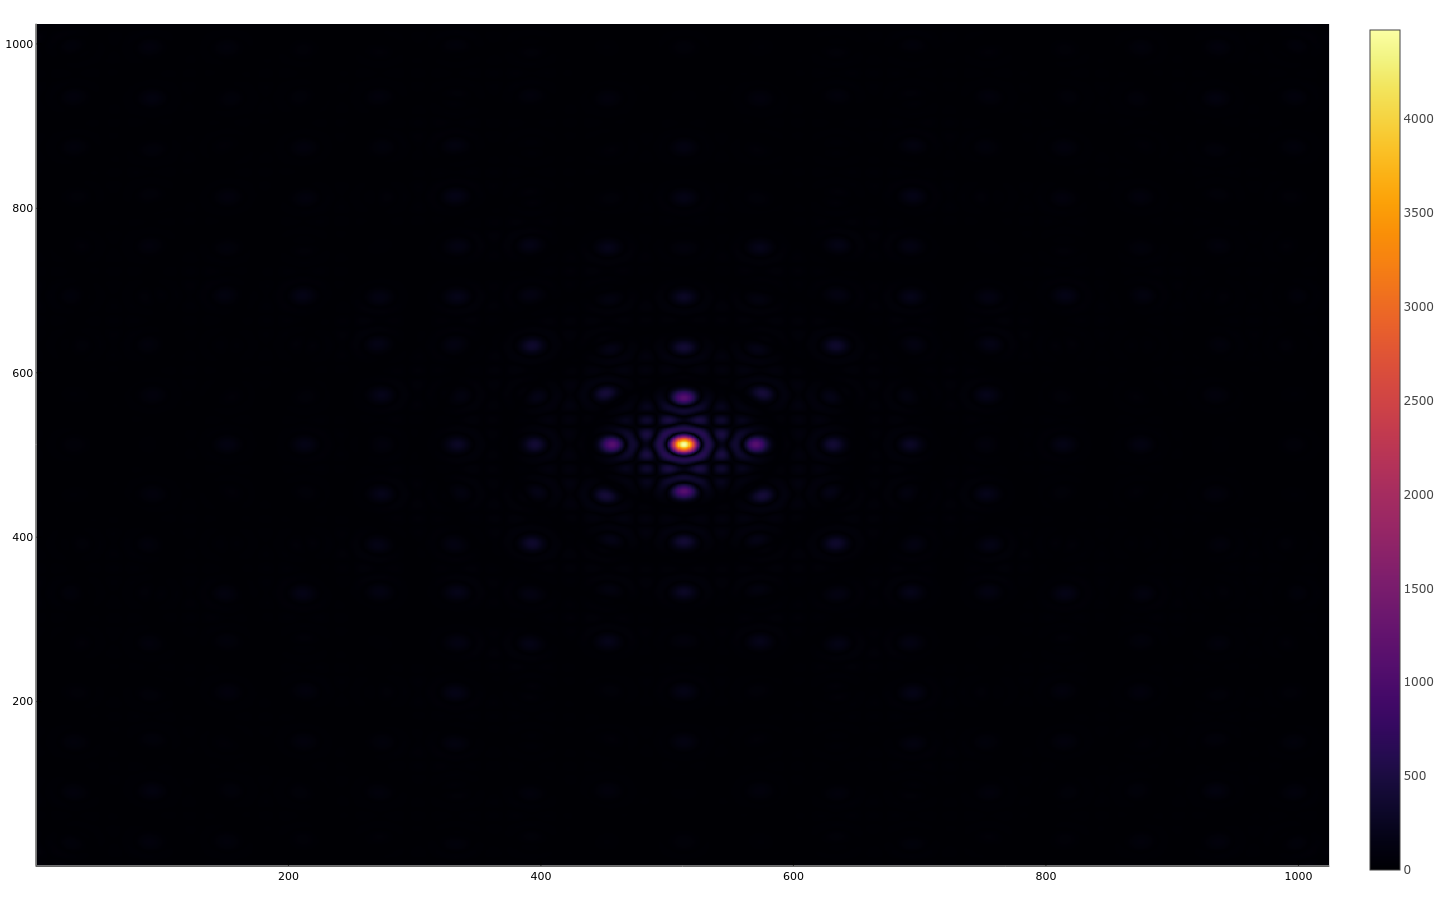
\includegraphics[width= \textwidth]{Figures/arraySim/sqr/circ_sqr_beamTop.png}
    \caption{Approximate beam shape of the square packed ultrasonic transducer array (Bore-sight view)}
    \label{fig:sqr_elem_topBeam}
    \end{minipage}
    
\end{figure}


\begin{figure}[ht!]
    \centering
    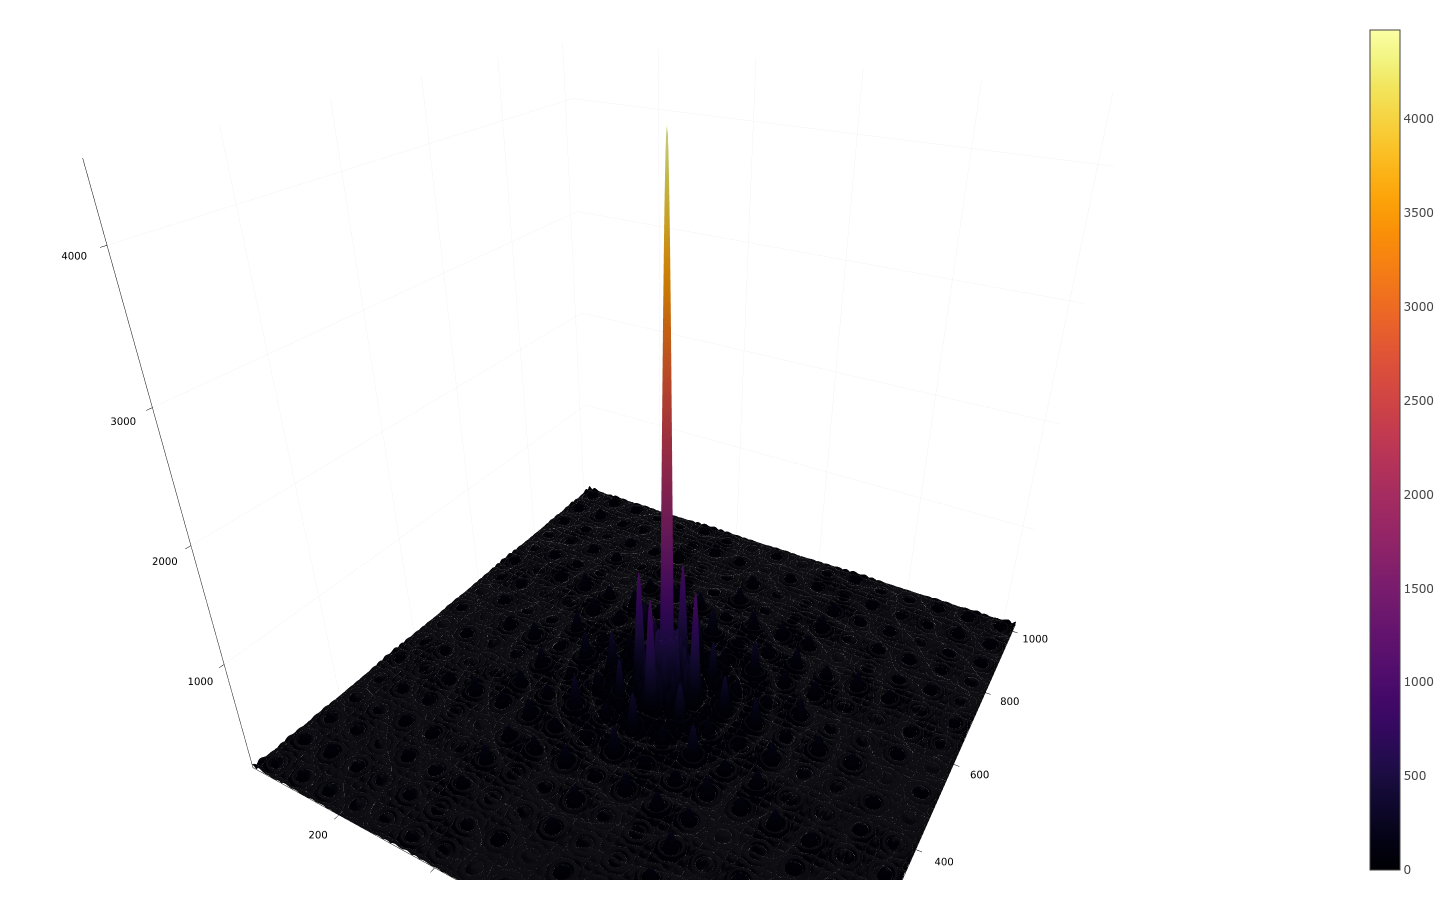
\includegraphics[width=0.8\textwidth]{Figures/arraySim/sqr/circ_sqr_beam3d.png}
    \caption{Approximate beam shape of square packed ultrasonic transducer array (3D view)}
    \label{fig:sqr_elem_3Dbeam}
\end{figure}

The simulation shows that when many evenly spaced transducers are used, it produces a less smooth beam shape due to the discontinuities between elements. For the square packed circular array the beam shape appears to have a significant center lobe with moderately larger side lobes in comparison to the single element simulated in figure \ref{fig:single_elem_3Dbeam}. Since this design has 21 elements, it would produce a larger sound pressure level at its peak than a single element, this proportion should be taken into consideration when deciding on the design.\\

The next simulation aims to reduce the spacing between transducer elements by use of a hexagonal packing as shown in figure \ref{fig:hex4.1}. This design has a filled fraction of 72.34\% which should yield a more uniform beam shape since the discontinuities between transducers have been reduced from the square packed design with a filled fraction of 66.37\% in figure \ref{fig:sqr4.5}. The magnitude of sound pressure energy in this design will be lower than the square design as it only has 19 elements instead of the 21 elements the square packed design contains.\\
The beam shapes were simulated for the hexagonally packed design and are presented in figures \ref{fig:hex_elem} to \ref{fig:hex_elem_3Dbeam}.

\begin{figure}[h!]
\centering

    \begin{minipage}{0.4\textwidth}
    \centering
    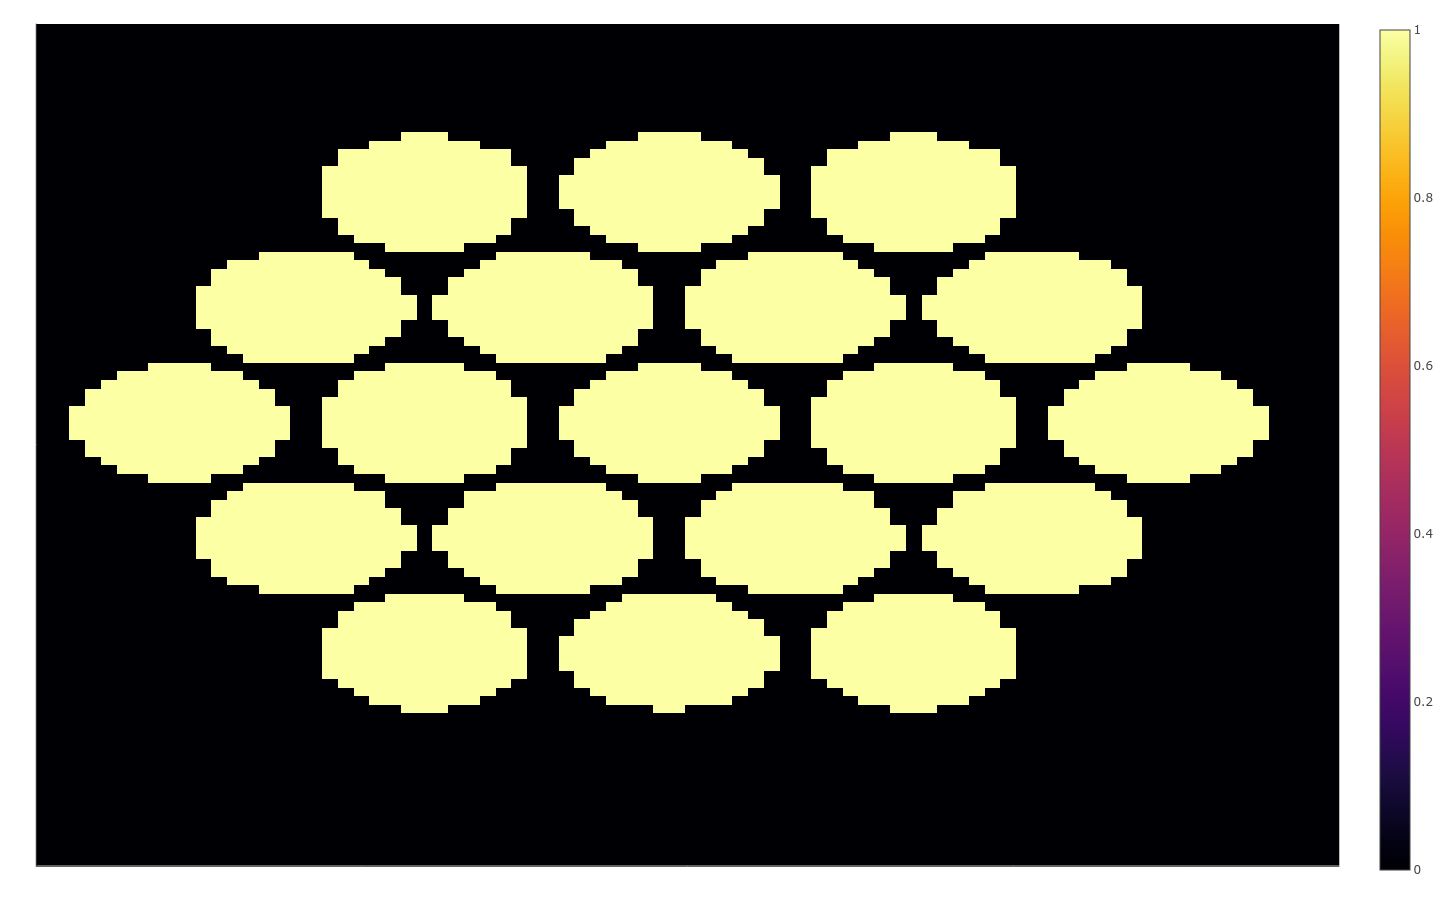
\includegraphics[width= \textwidth]{Figures/arraySim/hex/elemspacing.png}
    \caption{Hexagonally packed ultrasonic transducer elements to be modeled}
    \label{fig:hex_elem}
    \end{minipage}\hfill
    \begin{minipage}{0.4\textwidth}
    \centering
    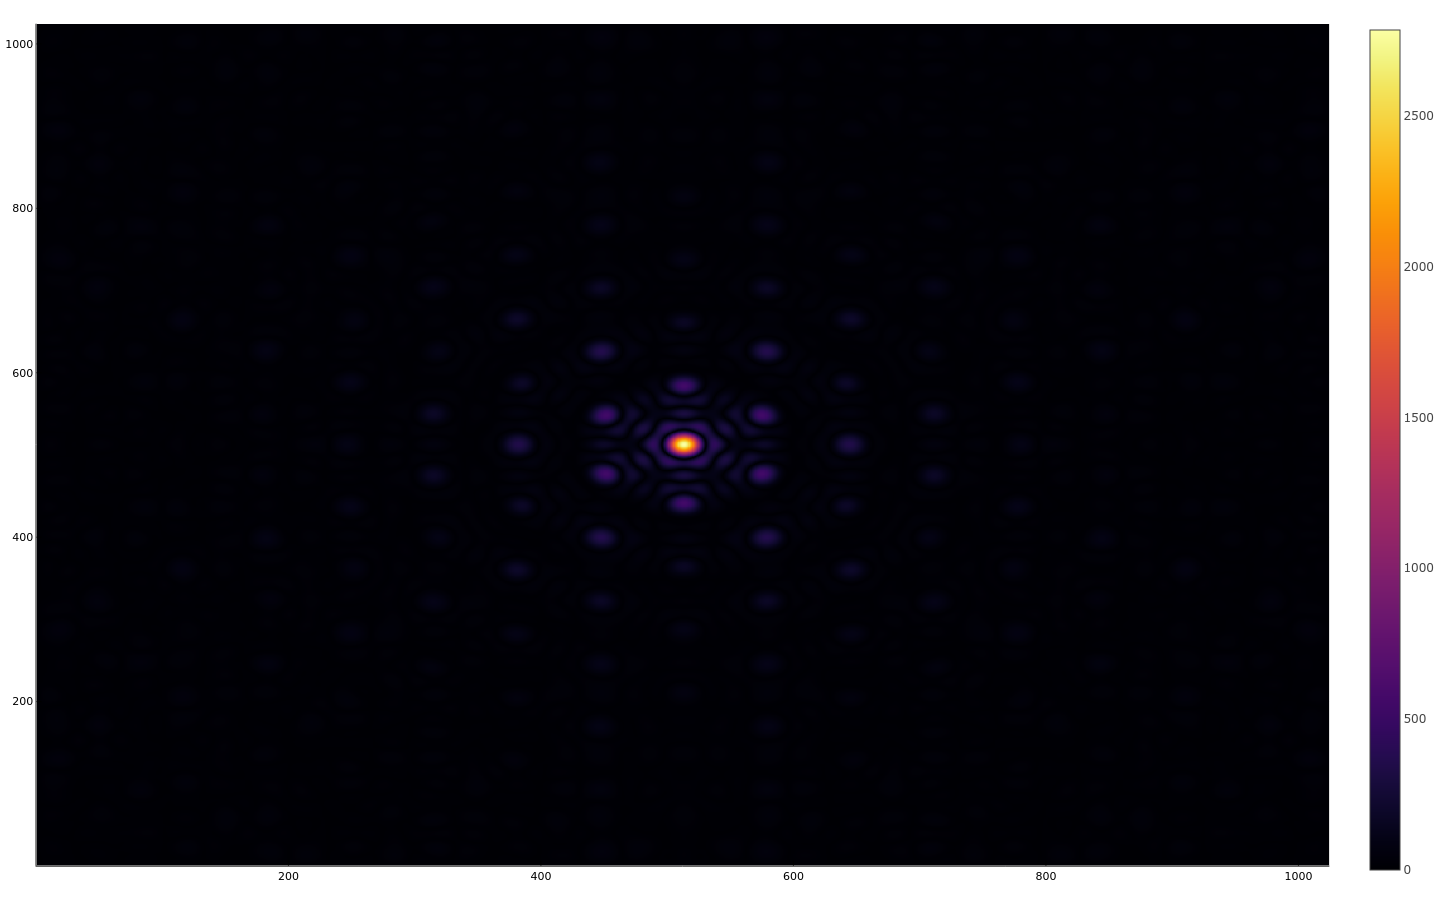
\includegraphics[width= \textwidth]{Figures/arraySim/hex/beampat(top).png}
    \caption{Approximate beam shape of the hexagonally packed ultrasonic transducer array (Bore-sight view)}
    \label{fig:hex_elem_topBeam}
    \end{minipage}
    
\end{figure}


\begin{figure}[ht!]
    \centering
    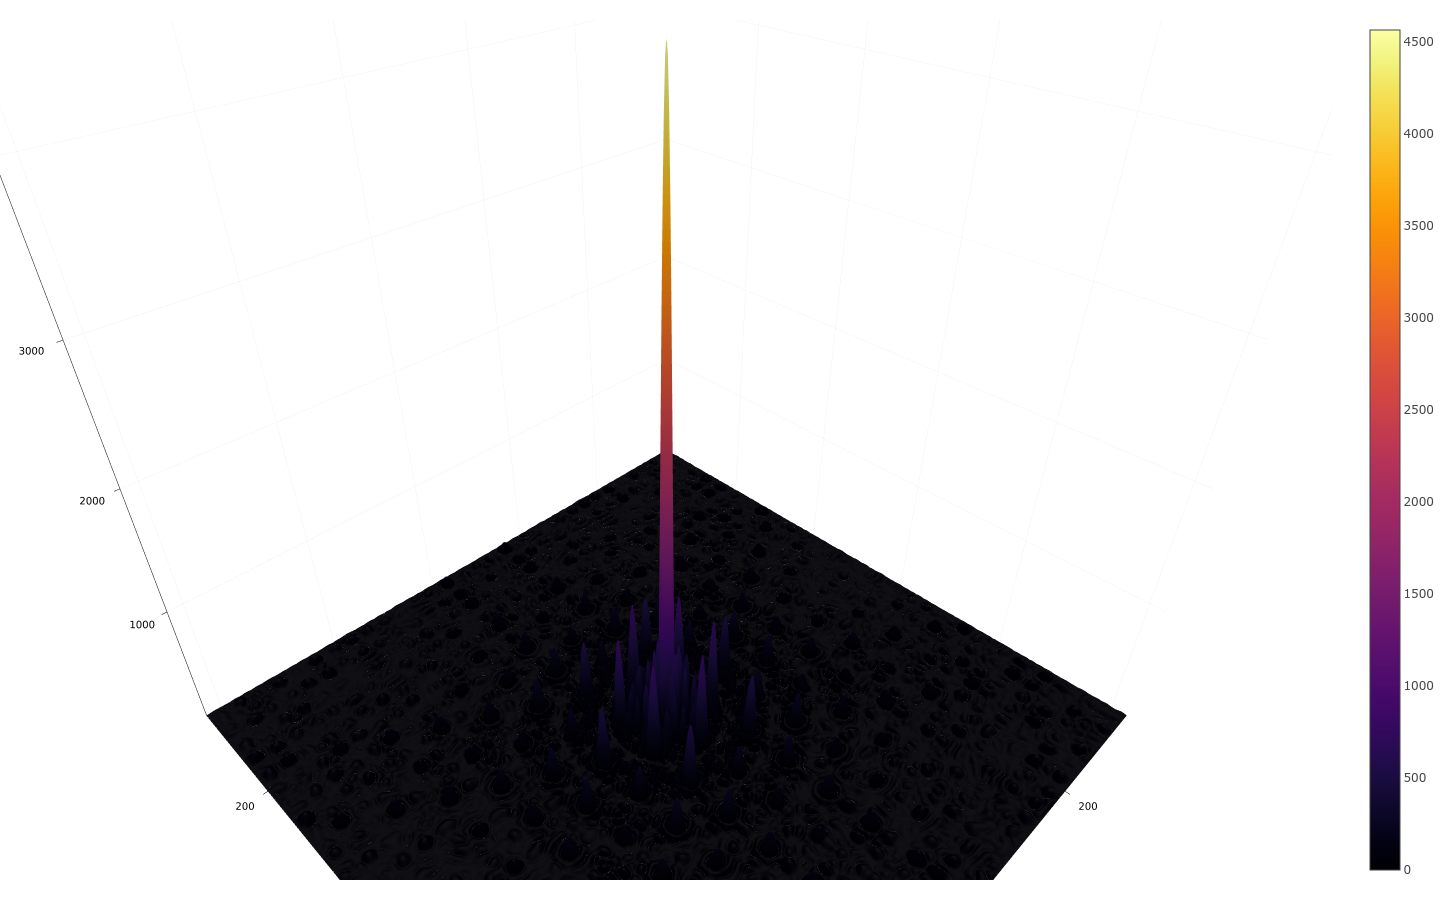
\includegraphics[width=0.8\textwidth]{Figures/arraySim/hex/beampat3dplaneview.png}
    \caption{Approximate beam shape of hexagonally packed ultrasonic transducer array (3D view) with scale}
    \label{fig:hex_elem_3Dbeamscale}
\end{figure}

\begin{figure}[ht!]
    \centering
    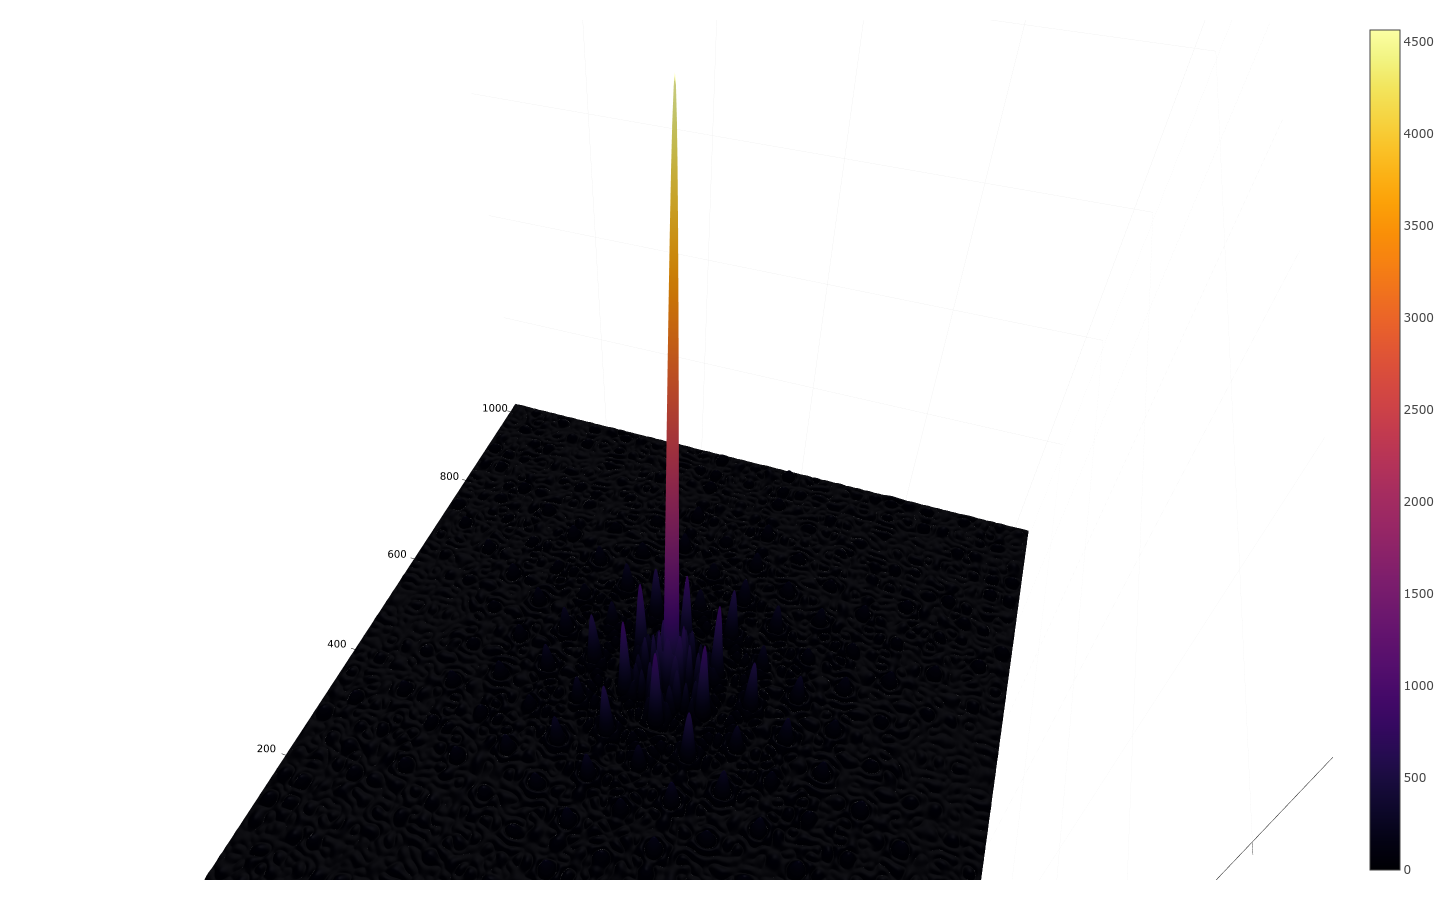
\includegraphics[width=0.8\textwidth]{Figures/arraySim/hex/beampat3d.png}
    \caption{Approximate beam shape of hexagonally packed ultrasonic transducer array (3D shifted view)}
    \label{fig:hex_elem_3Dbeam}
\end{figure}

It can be seen that more side lobes appear when using the hexagonal design, however it does better approximate a single transducer's beam shape with the relatively small lobes surrounding the large main lobe.
Both the square and hexagonal beam results indicate a similar peak relative magnitude of the main lobe of 4500, however; when analysing their bore-sight views the hexagonally packed array has six side lobes at approximate relative magnitude of 1000 while the square packed array has four side lobes with a relative magnitude of 1500. Neither result is fundamentally better than the other, but creating a beam with less side lobes would result in a more directive audio experience. Thus, since both results achieve a strong main lobe, the square packed solution is chosen going forward with the design as few side lobes is a more desirable trait for the directional audio system.
\newpage

\subsubsection{Array PCB design}
Prior to the array design simulations done in the previous section, some alternative array designs are considered in the interest of creating a modular PCB design. The rationale behind taking a modular approach is reduce the risk of failure due to faulty transducers. With a monolithic design, failure of a few transducers could risk damaging surrounding transducers while adding difficultly in troubleshooting where the failed components are. The transducers chosen for this design are the Kibitone 400ST ultrasonic transducers. A custom footprint for this transducer was created using the dimensions in its datasheet and used for the PCB design in KiCAD.

\begin{figure}[ht!]
    \centering
    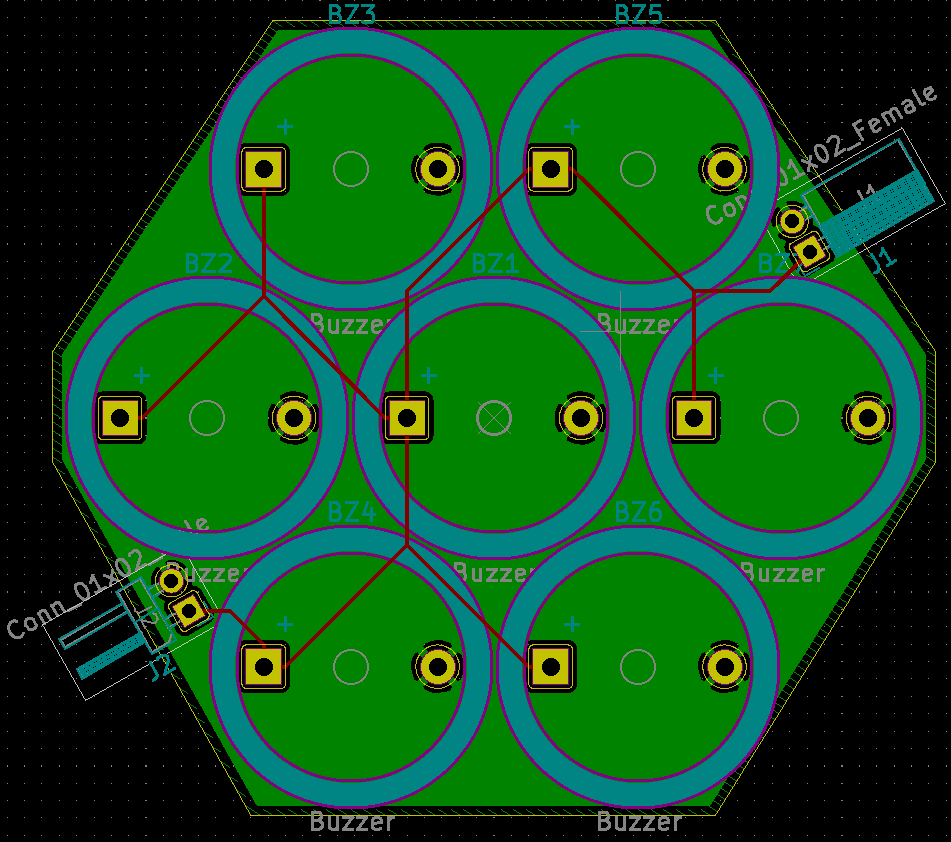
\includegraphics[width=0.6\textwidth]{Figures/Design/PCB/closeups/octogonalrev1.png}
    \caption{Rev 1.0 illustrating a modular octagonal design}
    \label{fig:modHex1.0}
\end{figure}

Figure \ref{fig:modHex1.0} demonstrates the first attempt at making a modular transducer array element. The idea behind this being that many hexagons can stack closely together providing minimal gaps between each PCB module. Rev 1.0 was used to estimate how best to layout the transducer and in what shape. This resulted in a octagonal design which only allowed 2 PCBs to interconnect as additional pin headers would be needed for a third module to link with the other two.

\begin{figure}[ht!]
    \centering
    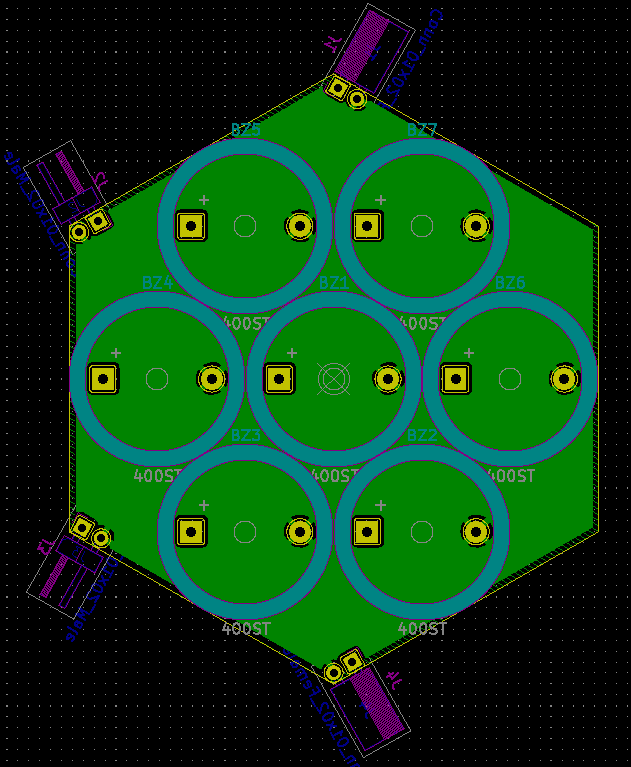
\includegraphics[width=0.6\textwidth]{Figures/Design/PCB/closeups/hexrev1.1.png}
    \caption{Rev 1.1 illustrating a modular hexagonal design with extra pin headers}
    \label{fig:modHex1.1}
\end{figure}

\begin{figure}[ht!]
    \centering
    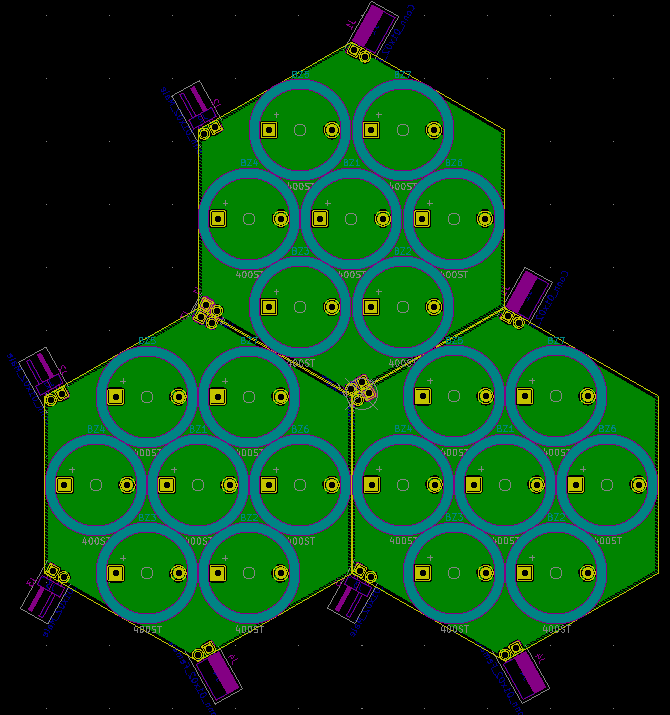
\includegraphics[width=0.6\textwidth]{Figures/Design/PCB/closeups/3xhex1.1.png}
    \caption{Three Rev 1.1 modular hexagonal PCBs interconnecting}
    \label{fig:3modHex1.1}
\end{figure}


Revision 1.1 is shown in figure \ref{fig:modHex1.1} where additional pin headers were added to allow up to three hexagonal PCB modules to connect to each other as demonstrated by figure \ref{fig:3modHex1.1}. Upon further development it was discovered that the male and female header pin placement was critical as exact alignment of them would be crucial for the modules to interconnect correctly with minimal gap. Adding to that, the centre of the array does not contain any transducers which would severely effect the uniformity of the beam. These factors drove the choice to redesign the array using a monolithic approach instead of modular and manage the risk faulty components by additional component level testing during the implementation stage.


\begin{figure}[ht!]
    \centering
    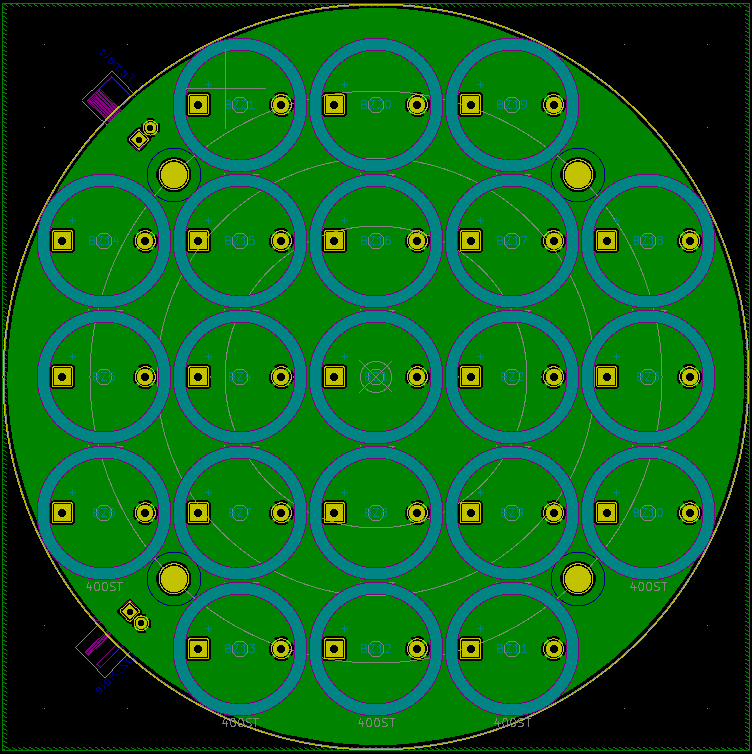
\includegraphics[width=0.8\textwidth]{Figures/Design/PCB/closeups/circCloserev1.2.png}
    \caption{Rev 1.2 monolithic design derived from packing simulations}
    \label{fig:CircMonoPCB}
\end{figure}

\begin{figure}[ht!]
\centering

    \begin{minipage}{0.49\textwidth}
    \centering
    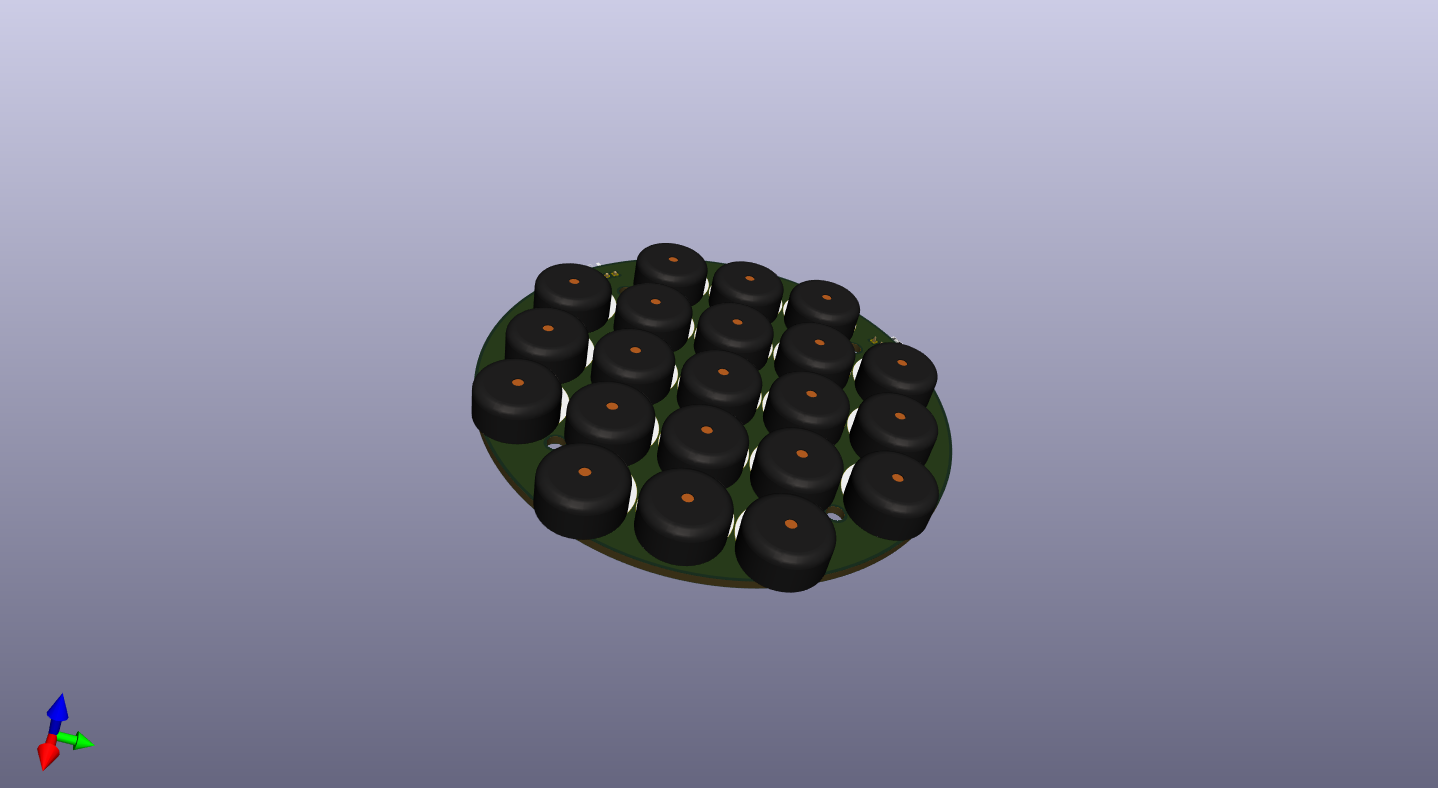
\includegraphics[width= \textwidth]{Figures/Design/PCB/Circular_Usonic_PCB_iso_3D.png}
    \caption{Isometric 3D view of Rev 1.2 Circular PCB design with square packing}
    \label{fig:isoPCB3D}
    \end{minipage}\hfill
    \begin{minipage}{0.49\textwidth}
    \centering
    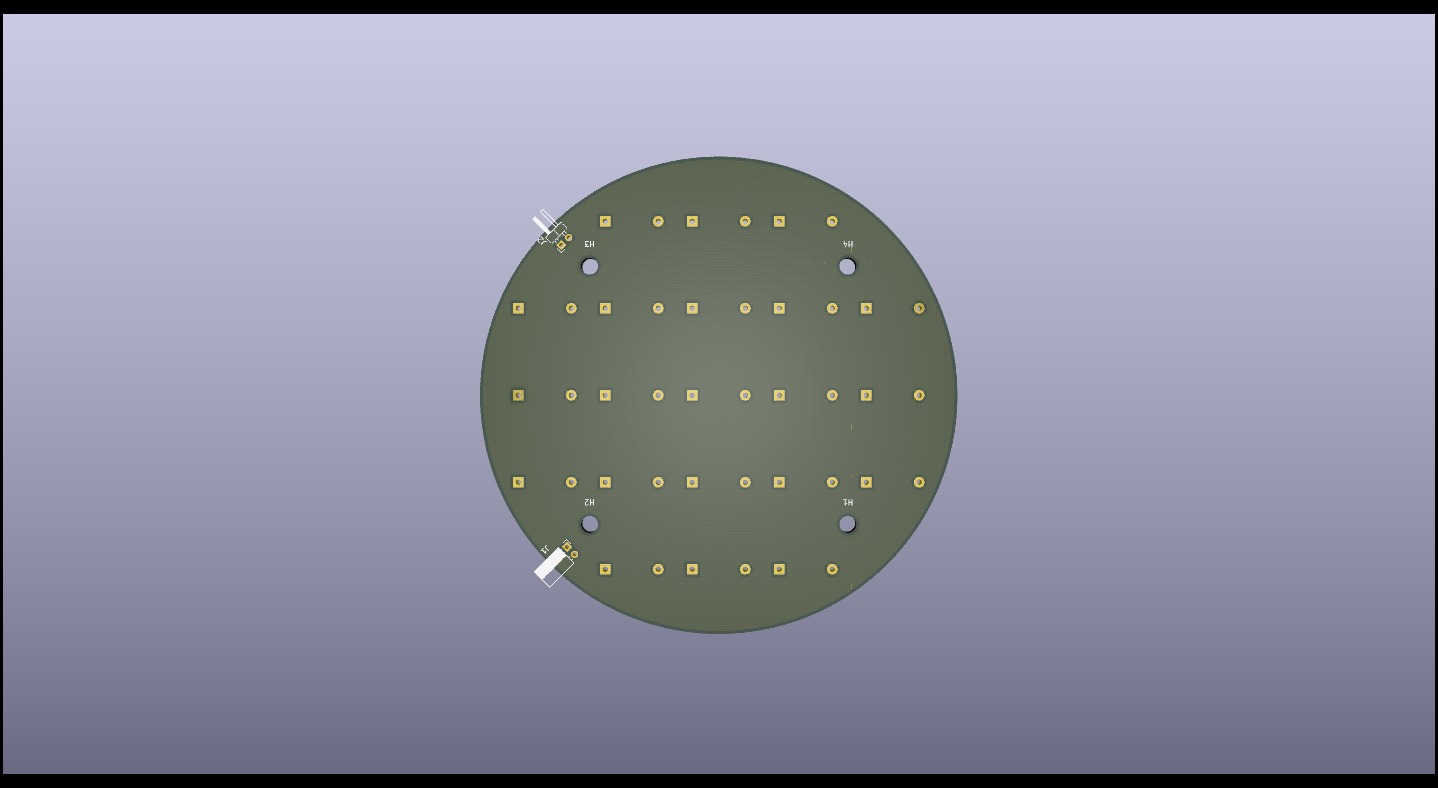
\includegraphics[width= \textwidth]{Figures/Design/PCB/Circular_Usonic_PCB_bot.png}
    \caption{bottom 3D view of Rev 1.2 Circular PCB design with square packing}
    \label{fig:botPCB3D}
    \end{minipage}
    
\end{figure}
\newpage
Learning from the packing and beam shape simulations done in the previous sections, a circular PCB with square packing was chosen for the PCB implementation. Figure \ref{fig:CircMonoPCB} illustrates the PCB design in KiCAD's PCB view while figures \ref{fig:isoPCB3D} and \ref{fig:botPCB3D} show the 3D view of the circular PCB featuring a radius of 4.5cm. Note the 3D views use plastic piezoelectric buzzers as their 3D model, this is due to the adaption and reuse of an existing buzzer when creating the custom PCB footprint for the Kibitone 400ST ultrasonic transducer. This PCB features four mounting holes for M4 screws simplifying the arrays ability to attach to a testing setup. Additionally two sets of pin headers are provided allowing the signal to be fed in while being measured on the other set of pin headers. 

\begin{comment}

Finally, the design choice was made to attach the first pin of each transducer to the front copper polygon pour while the second pin is attached to the back copper polygon pour. This allows the PCB to be as simple as possible and reduces the risk of failure due to a faulty trace. It does however potentially add some capacitance to the input on the PCB since the PCB now consists of two oppositely charged parallel plates. This value will be small in comparison to the front end capacitance of the amplifier which is in the order of 1000 $\muF$.
The approximate capacitance the PCB would create can be calculated using equation \ref{eqn:capEqn} where $\varepsilon_r$ is the relative permittivity of the PCB substrate and is usually around 4.5 and $d_layer$ is the distance between the layers which is approximately 2mm. This results in an approximate capacitance of 126.74pF for the circular PCB with a radius of 4.5cm which should have little effect.
%it actually has a big effect but shhhhh, I only just realised this causes the 1000uF cap to effectively add in parallel with this capacitance, reducing it down to 126pF which has a Xc of 33.046k, thus potentially increasing the impedance of the load beyond what the amplifier is designed for

\begin{equation}\label{eqn:capEqn}
    C = \varepsilon_0 \varepsilon_r \frac{\pi R^2}{d_layer}
\end{equation}
\end{comment}
